% THIS IS A LATEX TEMPLATE FILE FOR PAPERS INCLUDED IN THE
% *Anthology of Computers and the Humanities*. ADD THE OPTION
% 'final' WHEN CREATING THE FINAL VERSION OF THE PAPER. 
% DO NOT change the documentclass
%\documentclass[final]{anthology-ch} % for the final version
\documentclass{anthology-ch}         % for the submission

% LOAD LaTeX PACKAGES
\usepackage{booktabs}
\usepackage{graphicx}
% ADD your own packages using \usepackage{}

% TITLE OF THE SUBMISSION
% Change this to the name of your submission
\title{One Template to Rule Them All: Interactive Research Data Documentation with Quarto}

% AUTHOR AND AFFILIATION INFORMATION
% For each author, include a new call to the \author command, with
% the numbers in brackets indicating the associated affiliations 
% (next section) and ORCID-ID for each author.  
\author[1,2]{Moritz Mähr}[
  orcid=0000-0002-1367-1618
]
\author[1]{Moritz Twente}[
  orcid=0009-0005-7187-9774
]

% While we encourage including ORCID-IDs for all authors, you can
% include authors that do not have one by definining an empty ID.
% \author[2]{Author Three}[
%   orcid=
% ]

% There should be one call to \affiliation for each affiliation of
% the authors. Multiple affiliations can be given to each author
% and an affiliation can be given to multiple authors. 
\affiliation{1}{University of Basel, Switzerland}
\affiliation{2}{University of Bern, Switzerland}

% KEYWORDS
% Provide one or more keywords or key phrases seperated by commas
% using the following command
\keywords{open research data, documentation, reproducibility, Digital Humanities, Quarto, static sites, research data management, GitHub, Zenodo}

% METADATA FOR THE PUBLICATION
% This will be filled in when the document is published; the values can
% be kept as their defaults when the file is submitted
\pubyear{2025}
\pubvolume{1}
\pagestart{1}
\pageend{1}
\conferencename{Proceedings of Digital Humanities Tech Symposium (DHTech) at DH2025, NOVA University Lisbon}
\conferenceeditors{Editor1 Editor2}
\doi{00000/00000}  

\addbibresource{bibliography.bib}

%%%%%%%%%%%%%%%%%%%%%%%%%%%%%%%%%%%%%%%%%%%%%%%%%%%%%%%%%%%%%%%%%%%%%%%%%%%
% HERE IS THE START OF THE TEXT
\begin{document}

\maketitle

\begin{abstract}
This paper introduces the Open Research Data Template, a modular, Quarto-based framework developed to enhance the documentation, publication, and reuse of research data in the Digital Humanities. Originating from the Stadt.Geschichte.Basel project, the template addresses common challenges in research data management (RDM), such as poor documentation of data preprocessing and reuse pathways, by integrating narrative, metadata, and executable code into interactive, version-controlled websites. Built on \emph{The Turing Way} guidelines and leveraging GitHub for collaboration and Zenodo for archival DOIs, the template enables automated deployment, consistent repository structure, and living, reproducible documentation. Through diverse use cases, including project documentation, reproducible workflows, conference and teaching platforms, and living handbooks, the paper demonstrates the template’s flexibility and scalability. The authors argue that making robust, interactive documentation a default practice lowers technical barriers, improves sustainability, and fosters genuinely open and reusable research outputs. The widespread adoption of the template illustrates its value as a practical model for elevating open data standards and supporting the evolving needs of the Digital Humanities community.
\end{abstract}

\section{Introduction and Project Background}\label{introduction-and-project-background}

The large-scale research project Stadt.Geschichte.Basel at the University of Basel (2017--2026) aims to present Basel's history through a \href{https://emono.unibas.ch/stadtgeschichtebasel/}{ten-volume book series}, a \href{https://stadtgeschichtebasel.ch/}{digital portal}, and a dedicated \href{https://forschung.stadtgeschichtebasel.ch/}{research data platform}~\cite{goerlich2023}. Our team was tasked with managing a vast range of historical research data, from collection and organization to long-term preservation and public dissemination. Emphasis was placed on robust research data management (RDM) and continuous public engagement. We created an \href{https://dokumentation.stadtgeschichtebasel.ch/}{online documentation}~\cite{maehr2024g} as a virtual repository to make our work on Basel's historical data publicly accessible, ensuring the project maintained continuous public visibility and dialogue with future users even during development. Key RDM work packages included securing the project's diverse data (spanning images, maps, figures, tabular data, geodata, etc.) and developing interactive showcases for data presentation. Adhering to FAIR principles (Findable, Accessible, Interoperable, Reusable) was critical for reproducibility~\cite{wilkinson2016}, especially since historical scholarship to date lacks well-established discipline-specific RDM guidelines~\cite{hiltmann2018, ruediger2023}. We also adopted minimal computing tools like CollectionBuilder for digital collections, working with GLAM institutions to translate research data into formats accessible to the public~\cite{mahr2023g}. This comprehensive approach to RDM in a public history context underscored the need for better workflows to document not just the data, but also the processes and decisions behind the data~\cite{borgman2012}.

\section{Developing an Open Research Data Template}\label{developing-an-open-research-data-template}

To implement best practices across the research data lifecycle, we developed the \href{https://github.com/maehr/open-research-data-template}{Open Research Data Template}~\cite{mahr2023g} -- a modular, GitHub-based framework designed to streamline the publication, documentation, and reuse of open research data. The motivation arose from a common challenge: even as more datasets are shared openly, the \emph{preprocessing steps, methodological decisions, and potential pathways for reuse are often poorly documented}, rendering much ``open data'' difficult to actually reuse. Our template directly addresses this gap by enabling researchers (and our team) to package data with its context and code, not in isolation.

\textbf{Design Principles and Technologies:} The template is explicitly built around the guidelines from \href{https://book.the-turing-way.org/}{\emph{The Turing Way}}~\cite{theturingwaycommunity2025} to ensure that data and documentation are maximally reusable. It integrates \href{https://quarto.org/}{Quarto}, a modern scientific publishing platform, to enable \emph{executable documentation} that weaves together narrative, rich metadata, and live code in multiple languages. In practice, this means that within a single website, one can combine text with Python scripts, R analyses, Julia code, or even JavaScript visualizations (via Observable) -- all running in harmony to illustrate data workflows. Quarto's multi-language interoperability allows technical details and analyses to be directly embedded as interactive examples or dynamic outputs, ensuring that the documentation remains closely linked to the data and analysis.

We leveraged GitHub as both the development platform and the publishing infrastructure.\footnote{A migration to GitLab is technically feasible. Core repository data (files, history, issues, wikis) can be imported with low effort, but continuous integration workflows require a full rewrite of GitHub Actions into GitLab's \texttt{.gitlab-ci.yml}. Dependency updates, security scanning, and GitHub Pages equivalents also need reconfiguration.} Each project's repository can be based on the template, benefiting from automated version control and collaboration. GitHub Actions (continuous integration workflows) handle routine tasks such as building the site, running tests (e.g., linting, validating links, generating changelogs, etc.), and deploying updates to GitHub Pages for hosting. This means that when contributors push changes (for example, updating a dataset or its analysis code), the website regenerates automatically, ensuring the latest information is always live without manual intervention. The template also integrates with \href{https://zenodo.org/}{Zenodo} for long-term archiving: whenever a project using the template is ready to publish a snapshot (for instance, alongside a paper or at a project milestone), a Zenodo deposit can be generated, minting a DOI for that version. This guarantees both accessibility and citability for the materials, as datasets and documentation snapshots receive persistent identifiers. By combining static webpages with archival DOIs, the template bridges the gap between ephemeral project websites and permanent scholarly records.

\begin{figure}[t!]
  \centering
  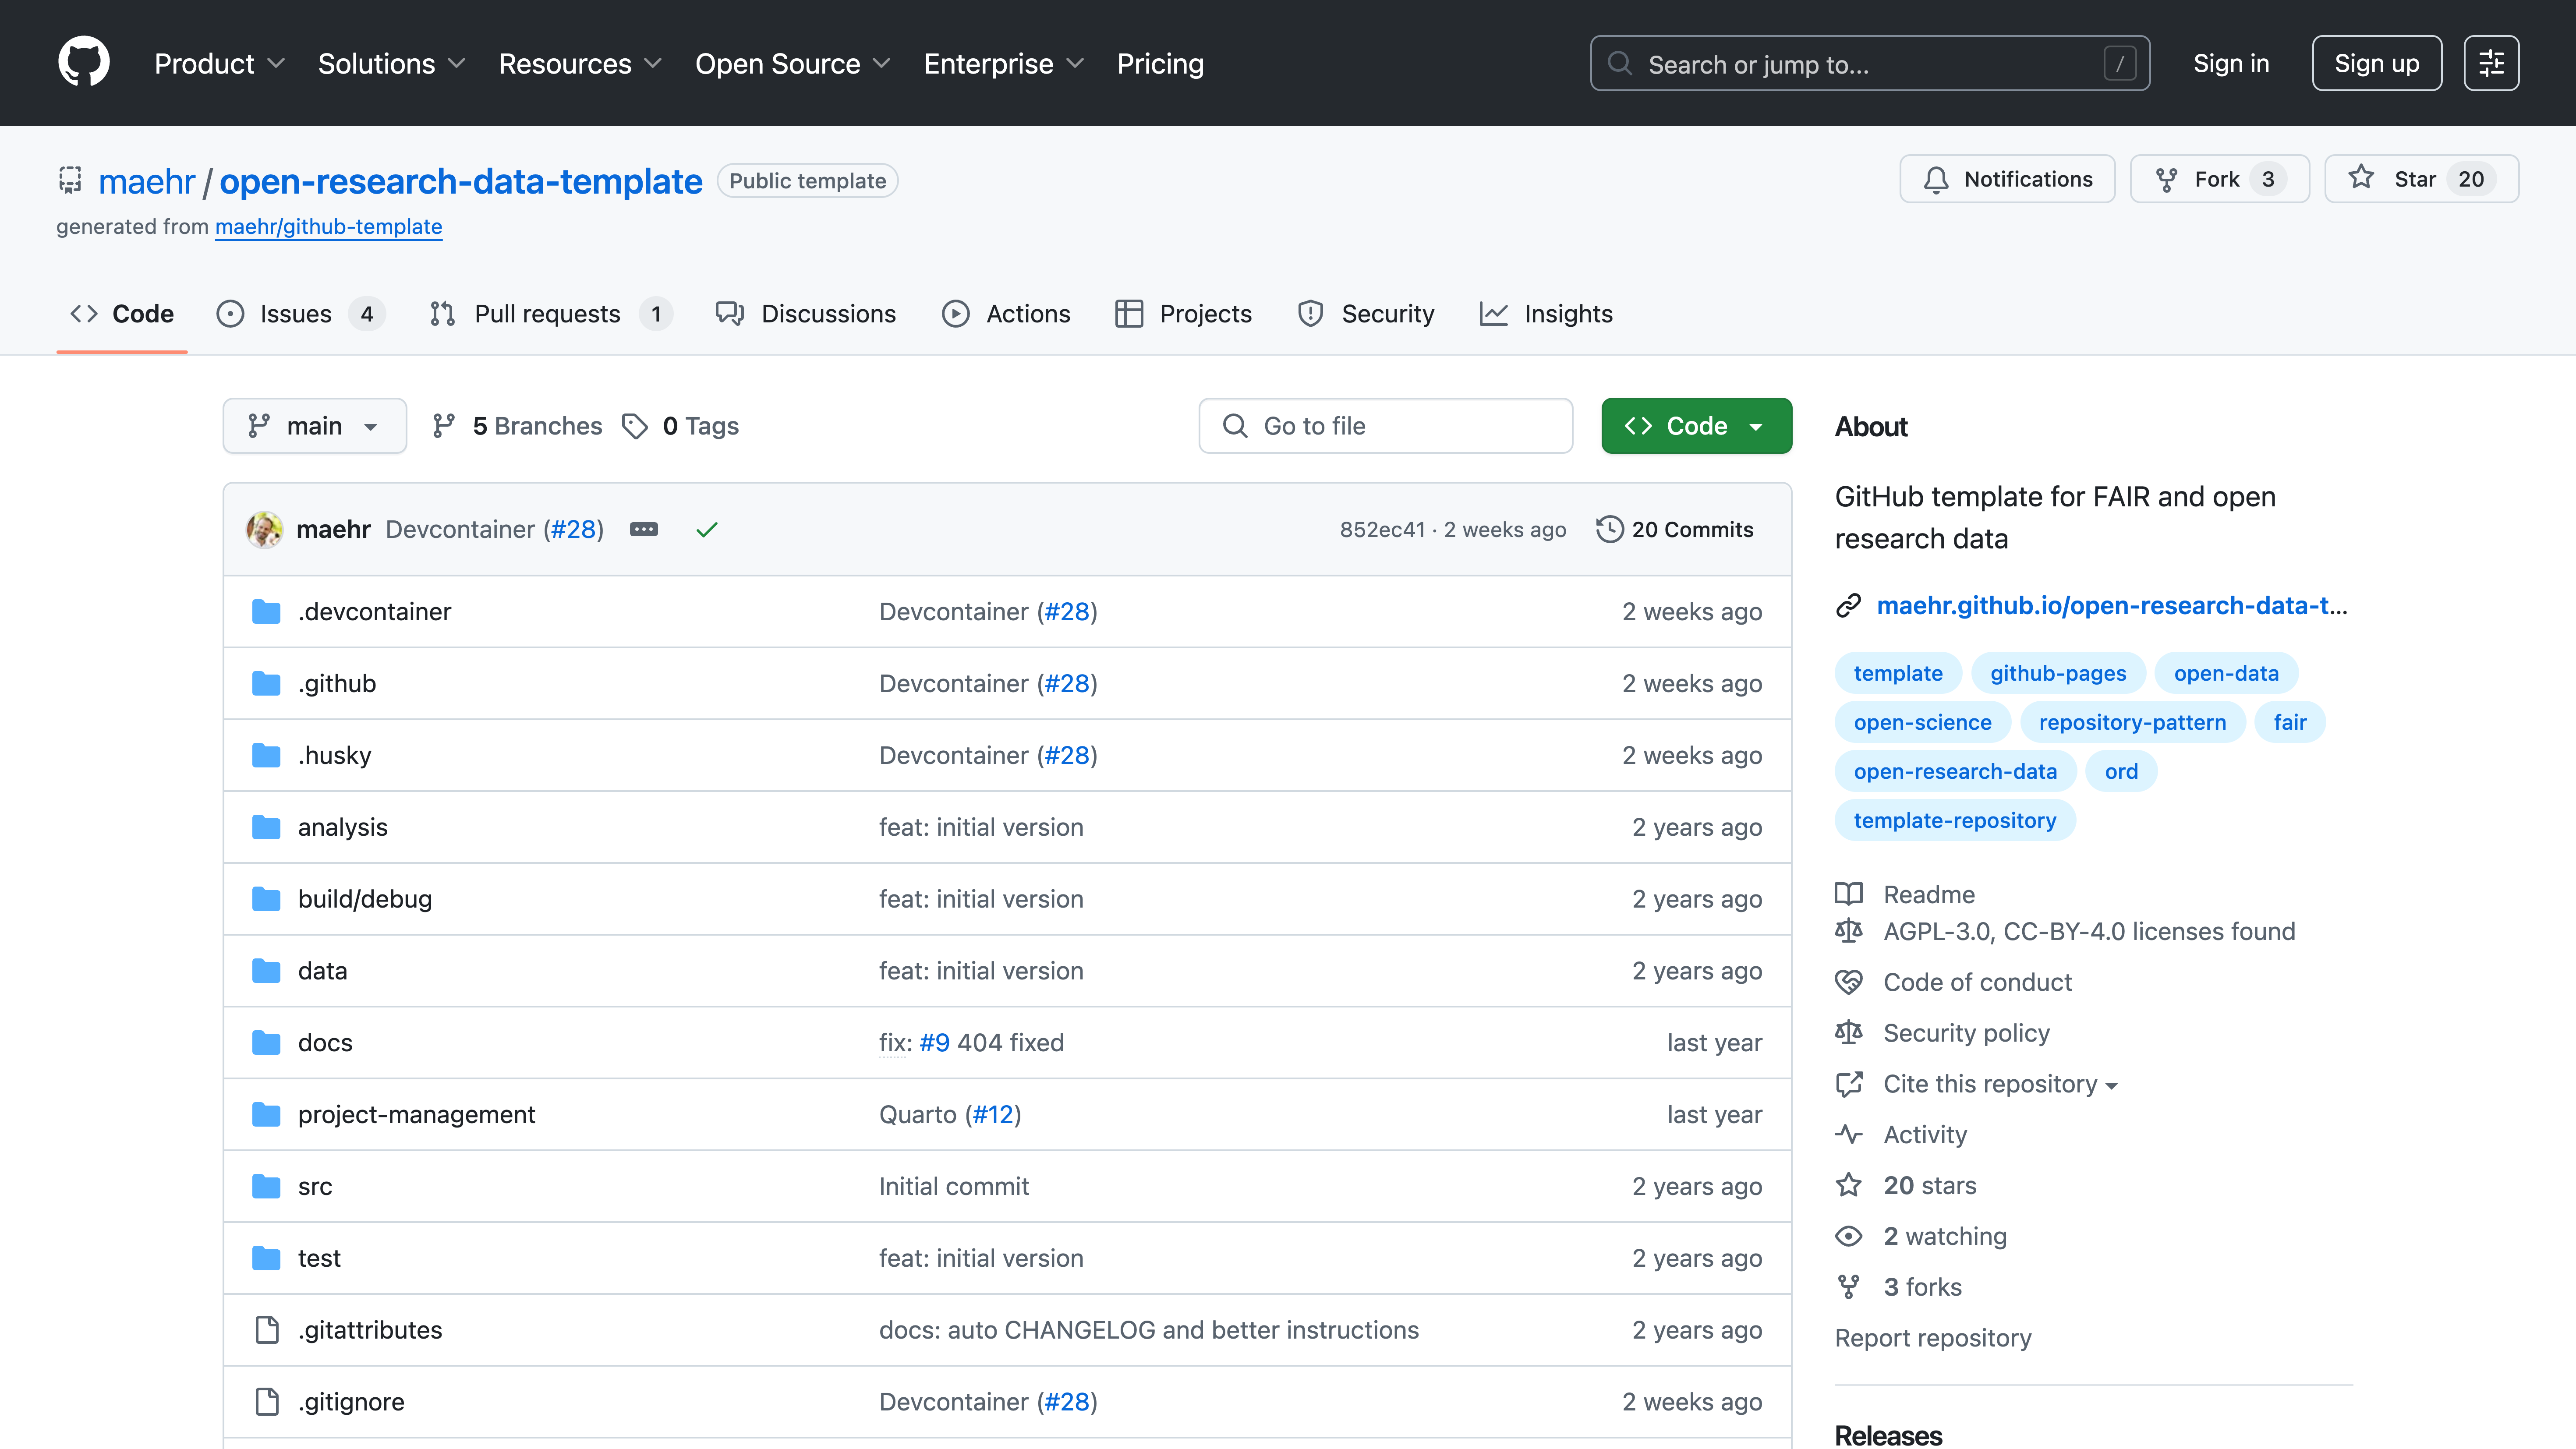
\includegraphics[width=0.45\linewidth]{images/open_research_data_template.png}
  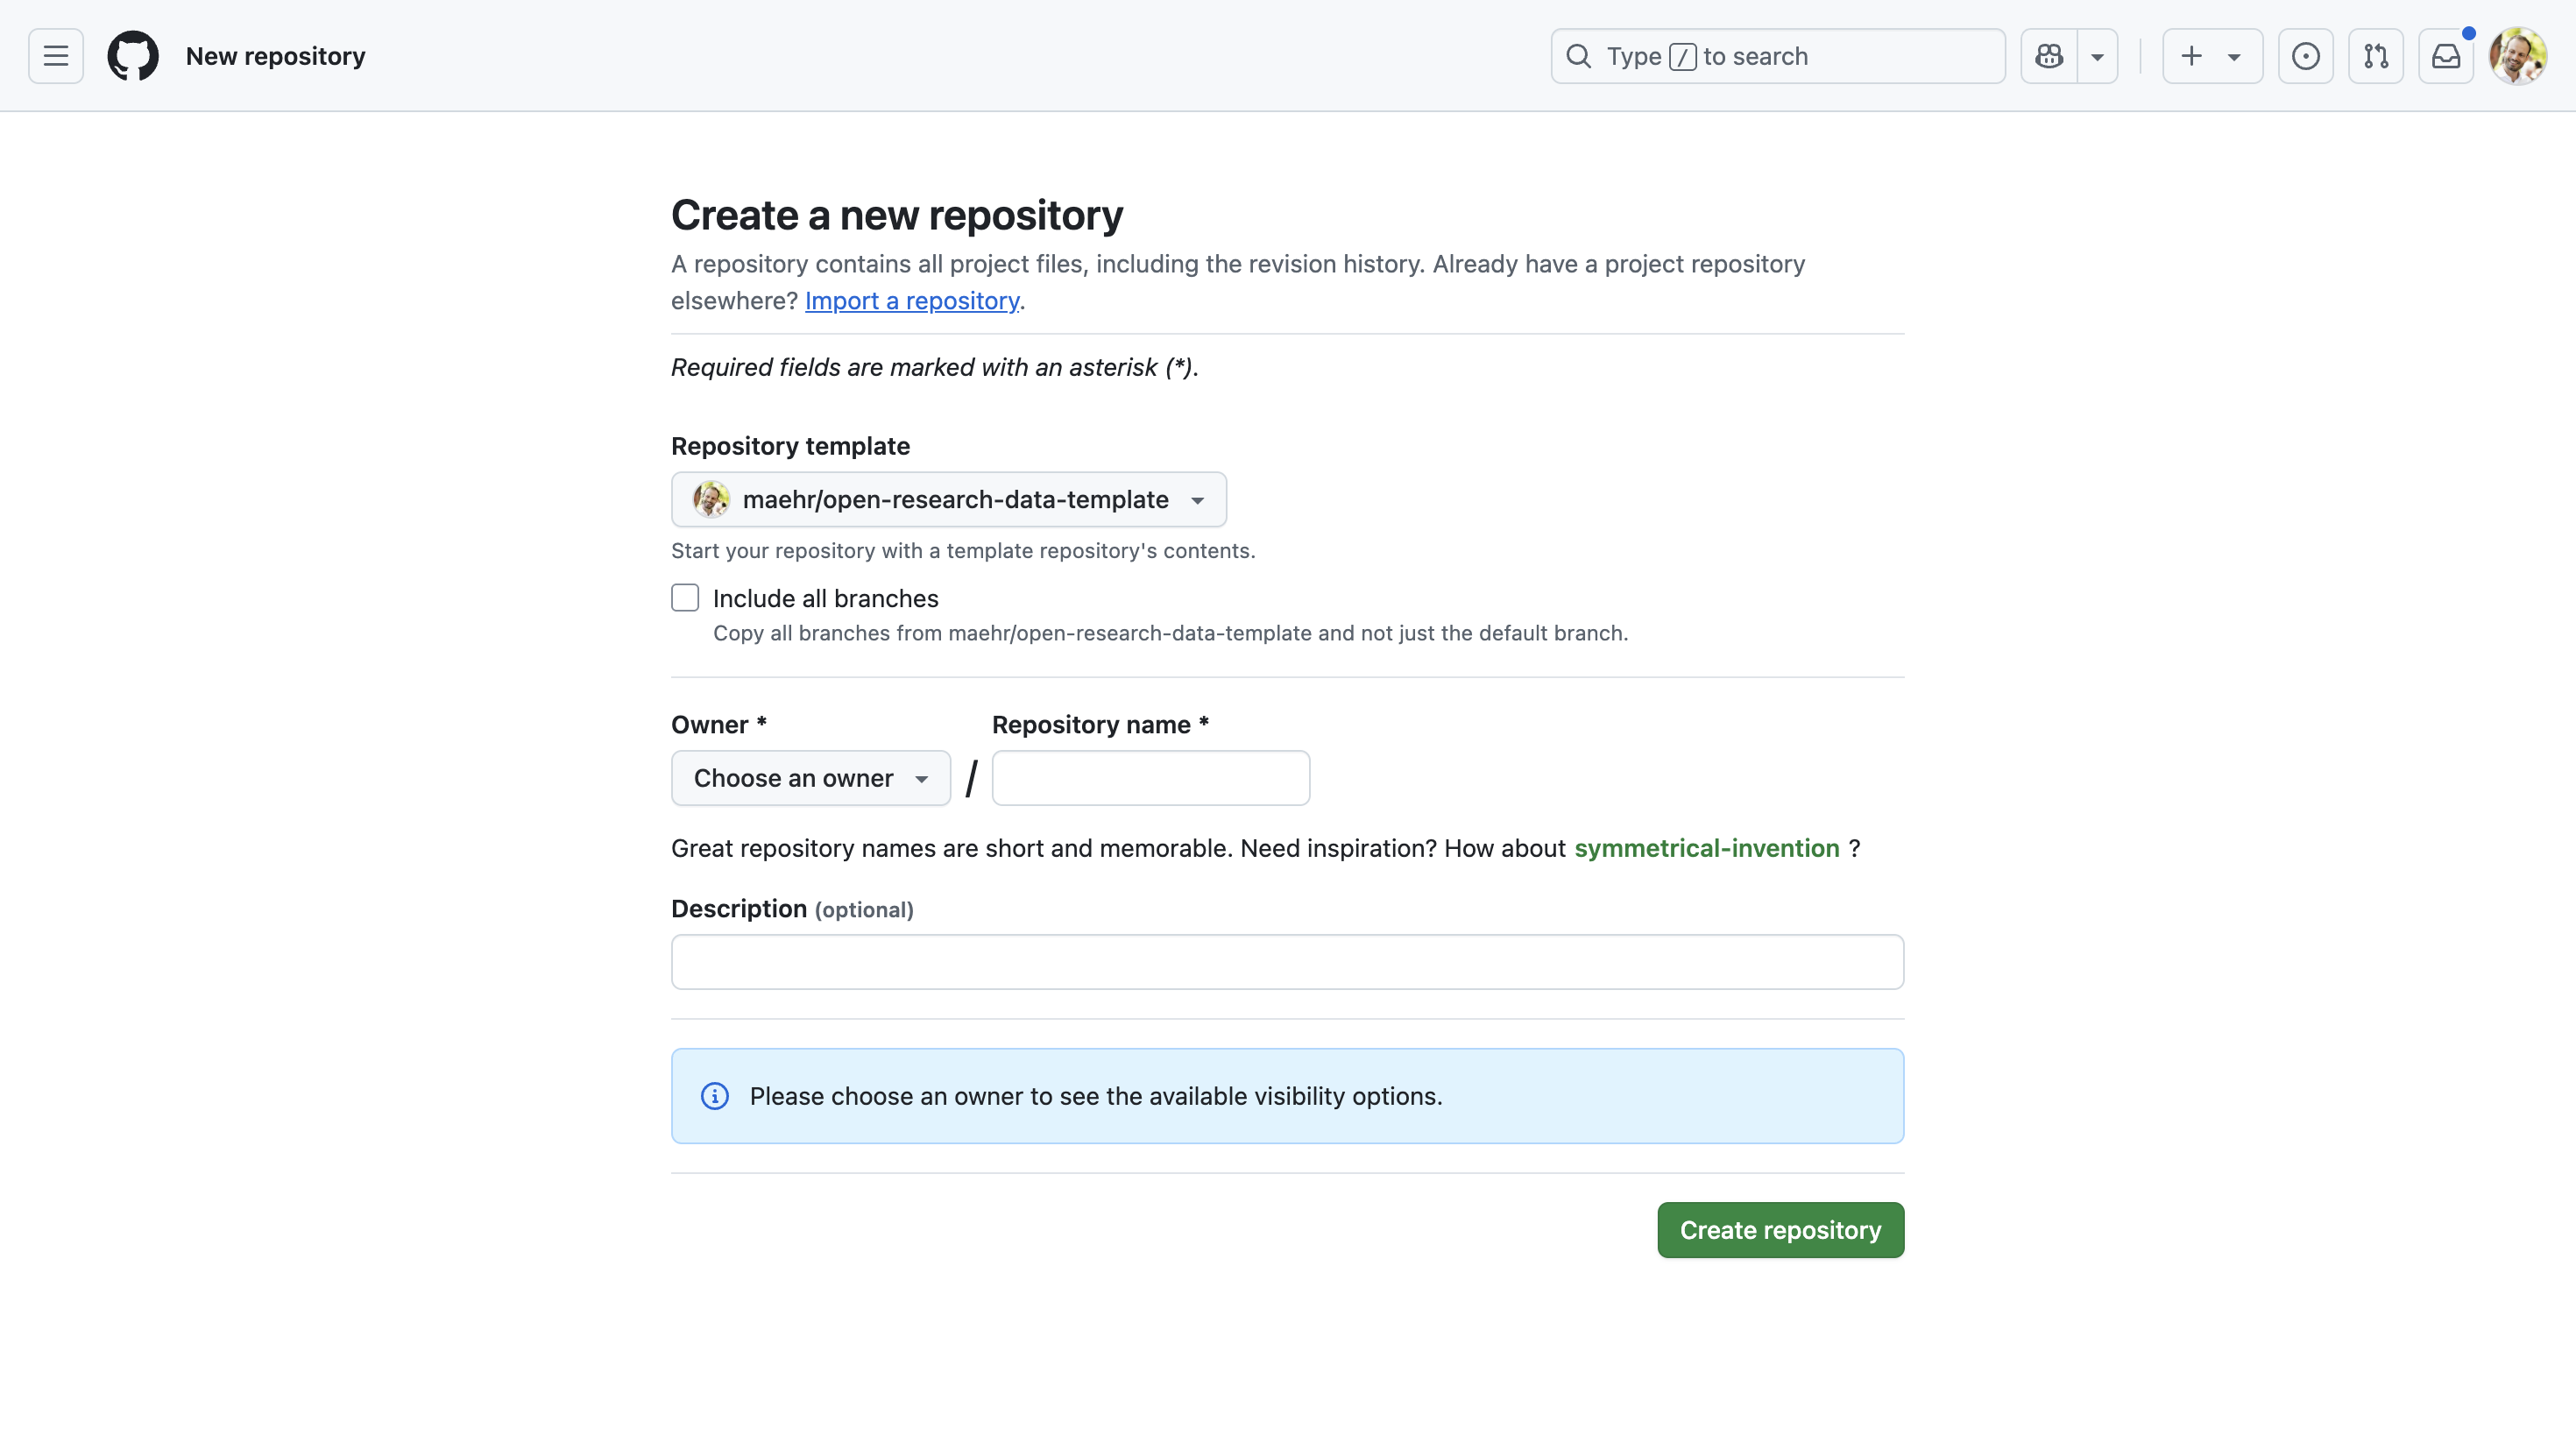
\includegraphics[width=0.45\linewidth]{images/open_research_data_template_new_repo.png} \\
  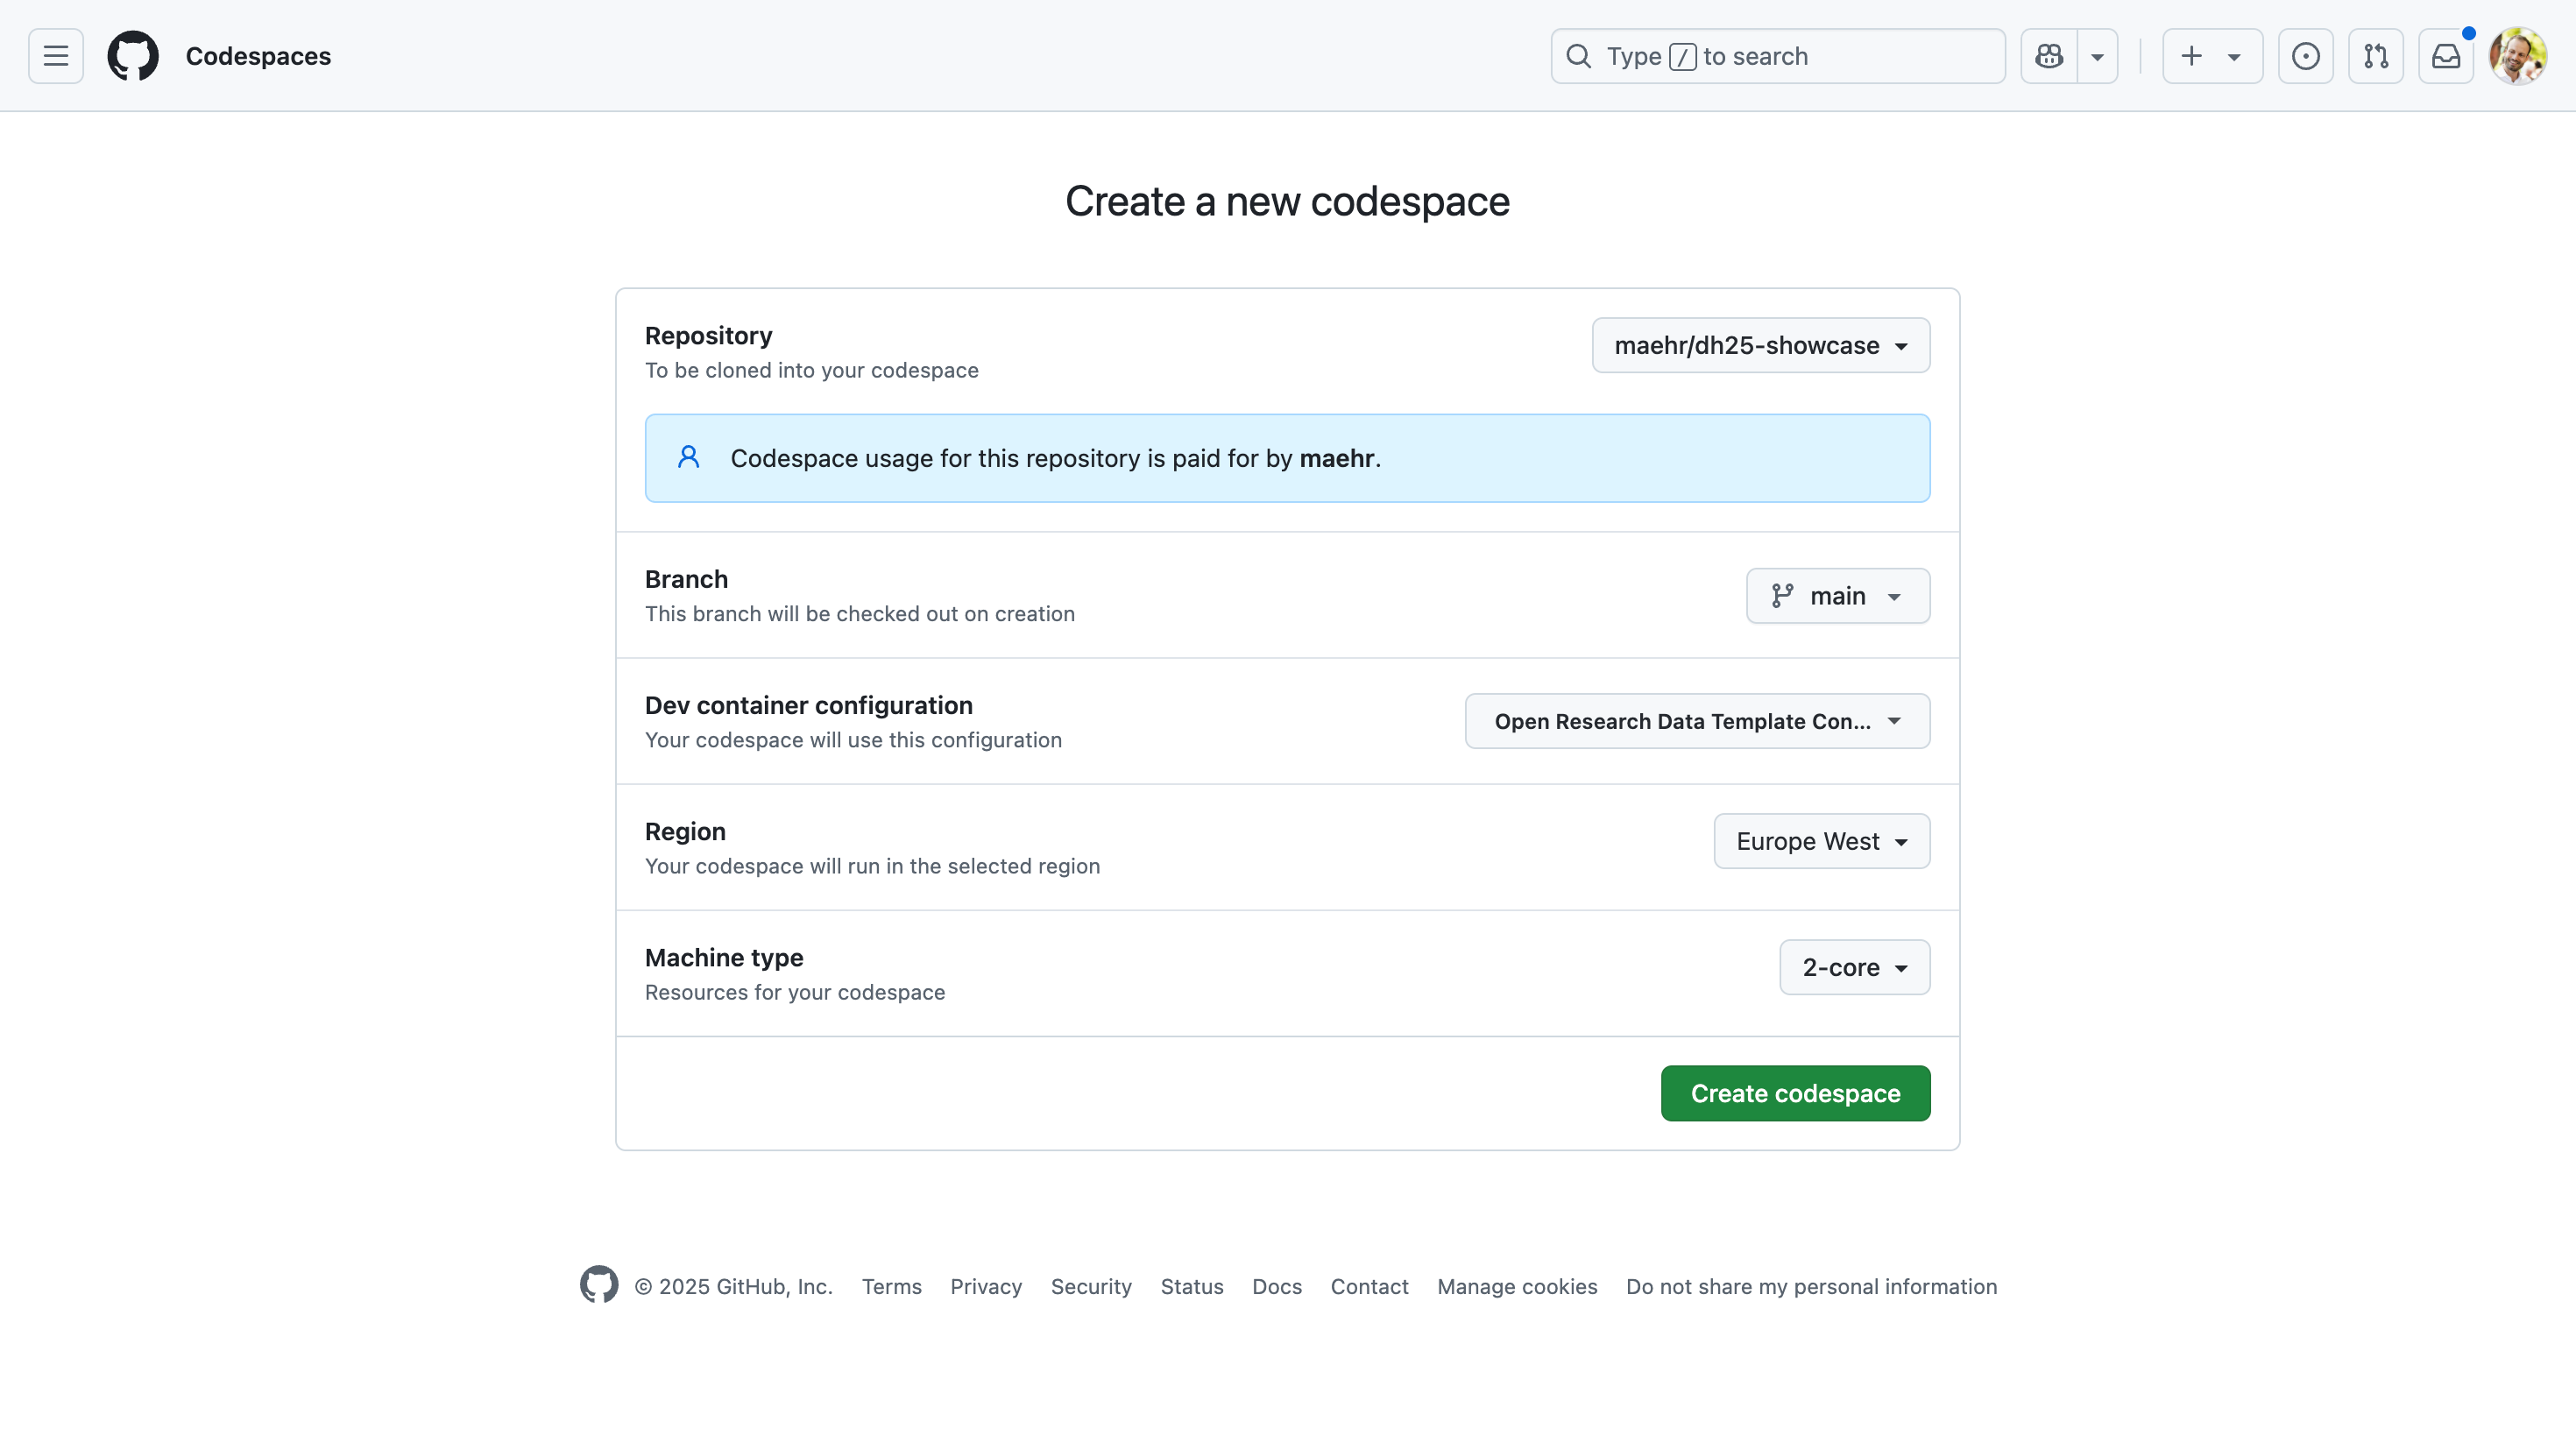
\includegraphics[width=0.45\linewidth]{images/open_research_data_template_codespace.png}
  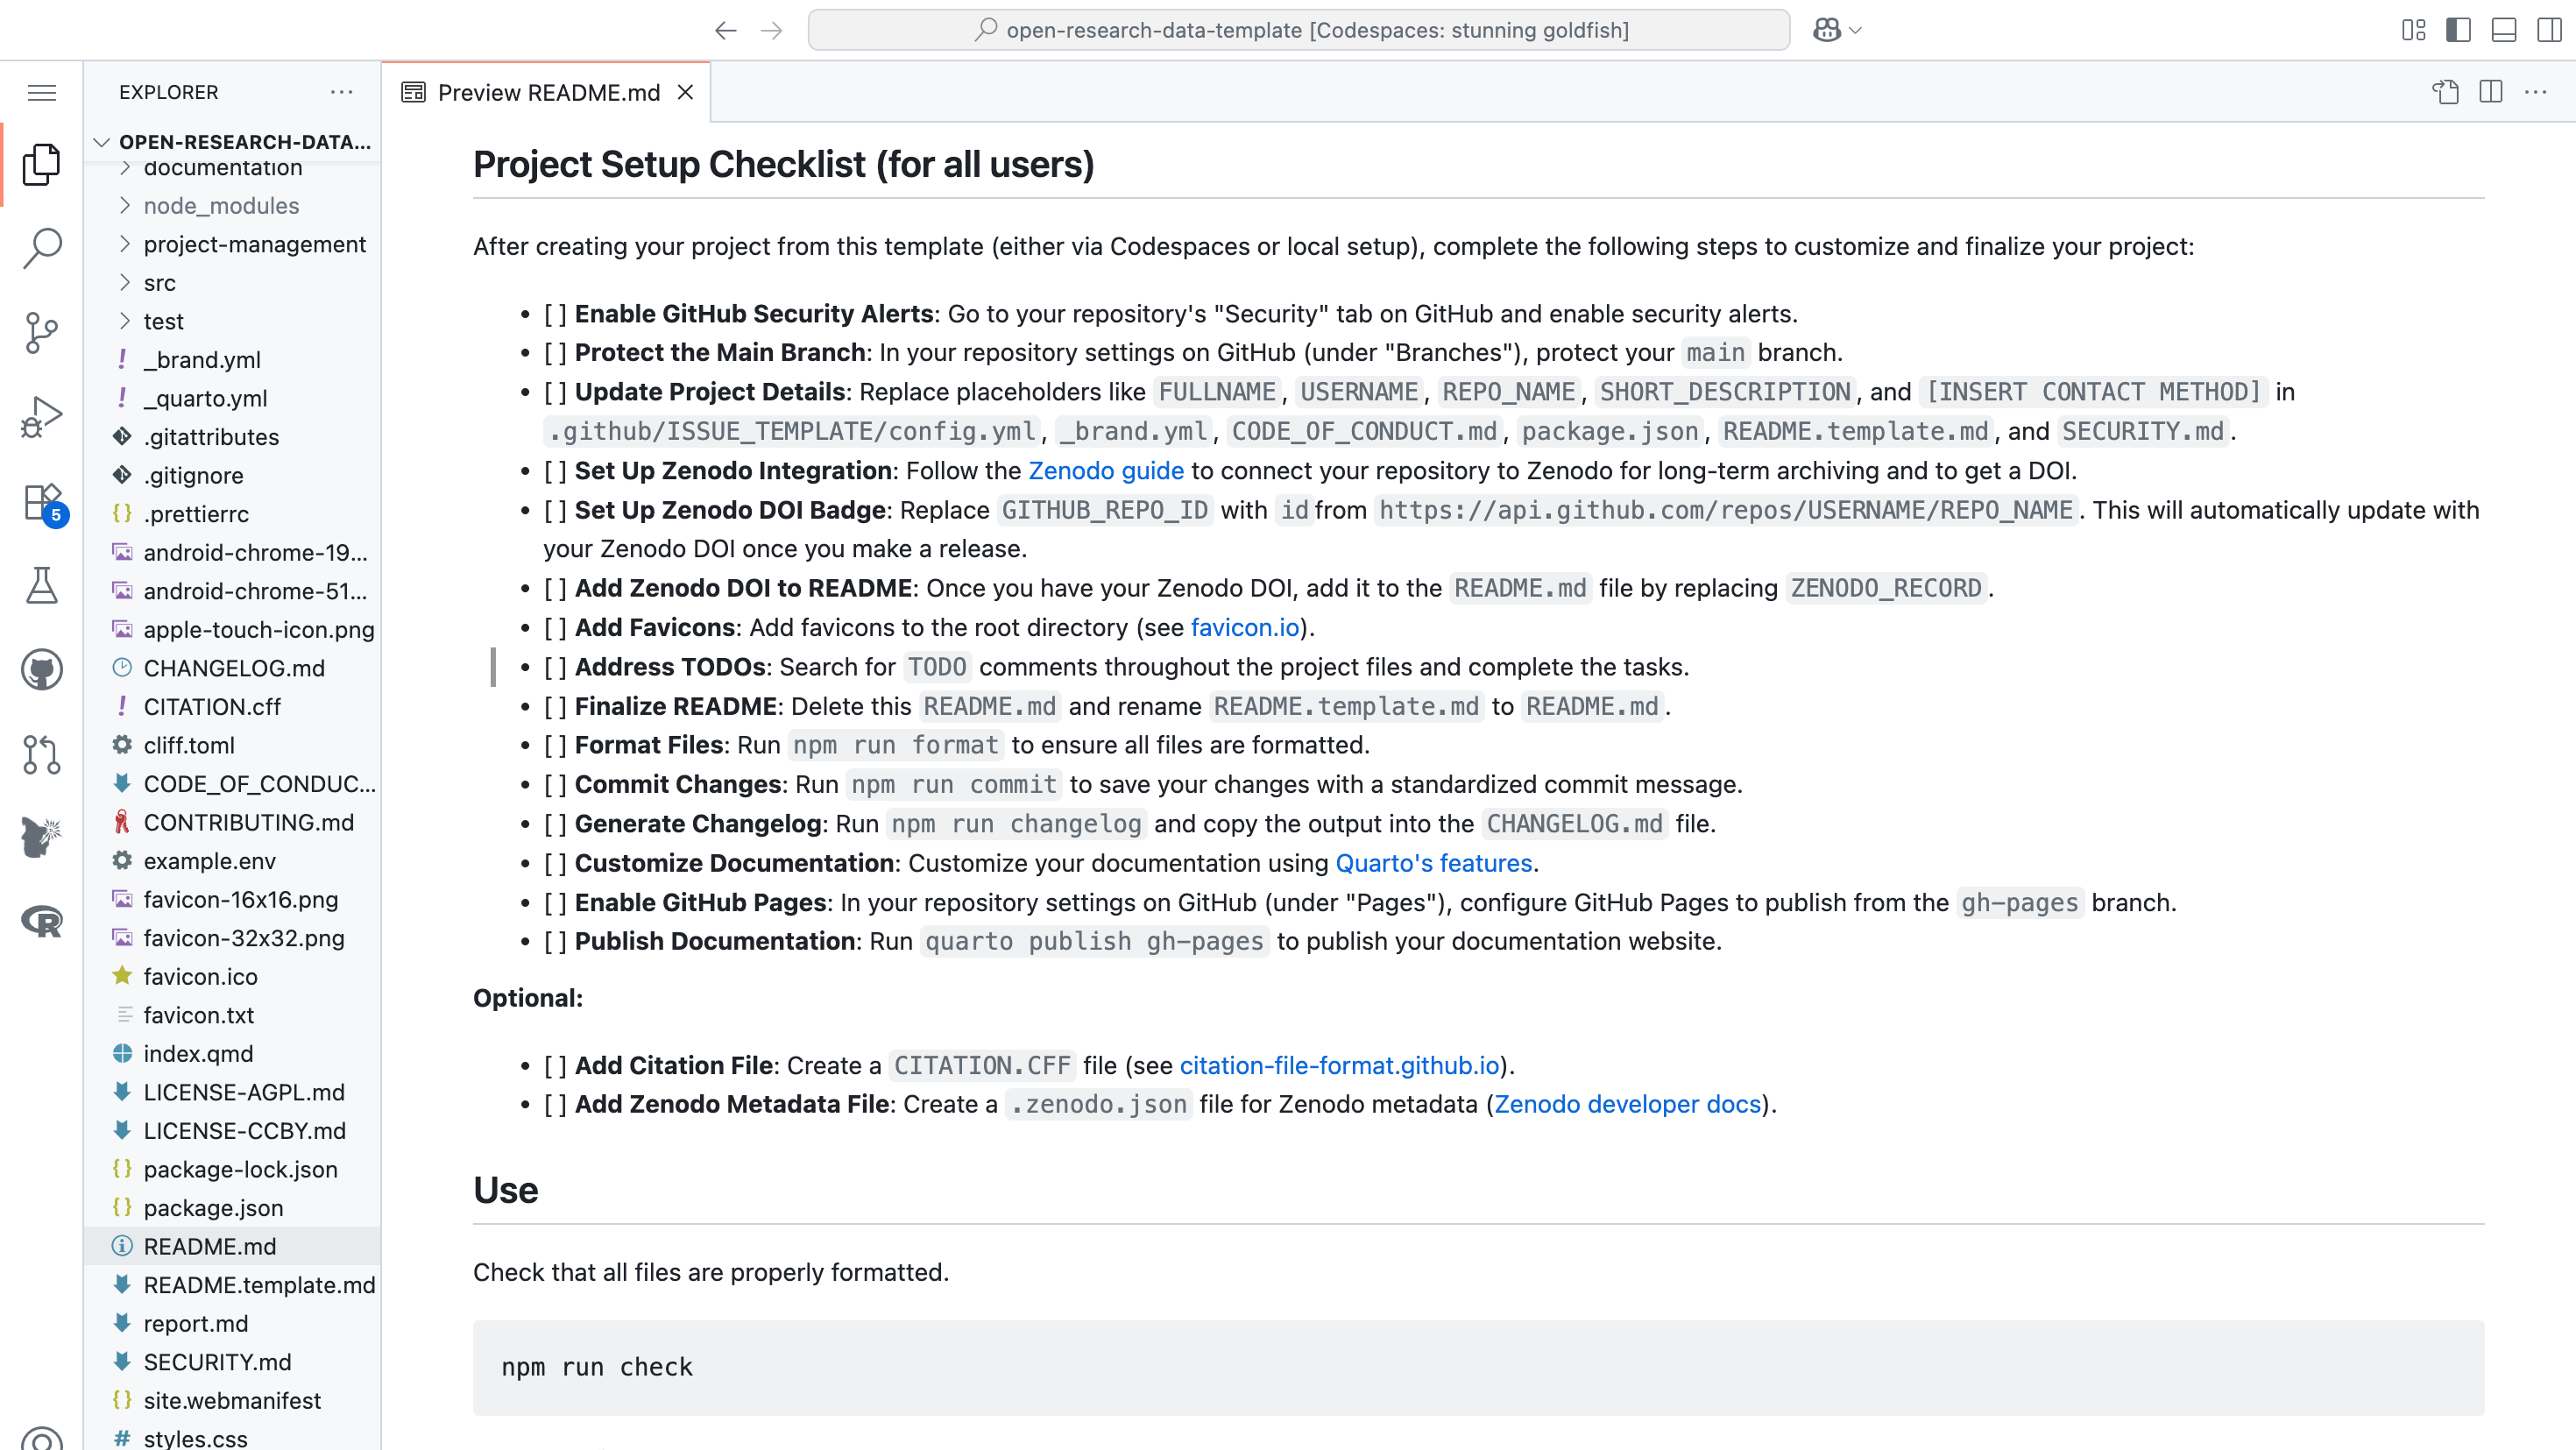
\includegraphics[width=0.45\linewidth]{images/open_research_data_template_readme.png}
  \caption{Setup and structure of the \emph{Open Research Data Template} repository, demonstrating how to create a new repository, open it in a codespace, follow the setup checklist, and explore the repository contents.}
  \label{fig-open-research-data-template}
\end{figure}

A key innovation of our approach is treating documentation as a living, executable environment rather than a static afterthought. Traditionally, projects might release data as supplementary files and methods as PDF documentation, but our template merges static metadata, narrative descriptions, and executable code into a single integrated and interactive website. This ensures that data, methods, and results remain interconnected and in context~\cite{rule2019}. Anyone revisiting the project can not only read about what was done but also see (and run) the actual code that produced the results, all within the documentation. This transparency lowers barriers to reuse: a future researcher can reproduce or adapt the workflow in their environment, confident that nothing is lost in translation. In essence, the template turns what would be static data archives into ``living, extensible resources,'' continuously usable and updatable beyond the original project.

\textbf{Features and Best Practices:} The Open Research Data Template comes with a set of best practices built in. It enforces a standardized, logical repository structure for organizing data, code, and content, building on \emph{The Turing Way} handbook on reproducible research~\cite{theturingwaycommunity2025}. Key features include:

\begin{itemize}
\tightlist
\item
  \textbf{Executable Narratives:} Authors can create documents that directly incorporate code outputs (tables, plots, maps, etc.) into the narrative. Quarto's support for Jupyter and other kernels means the documentation itself can regenerate analyses if data or parameters change. This ensures that analysis results and figures are always in sync with the latest data and code, exemplifying reproducible research practices.\\
\item
  \textbf{Automated Deployment and Testing:} By using continuous integration, the template reduces the technical overhead for researchers. For example, when writing documentation in markdown or Jupyter notebooks, authors simply commit their work; the template's GitHub Actions pipeline then automatically runs any code (in a controlled environment), builds the static site, checks for issues, and publishes it. This encourages frequent updates and iterative improvement without requiring web development expertise.\\
\item
  \textbf{Integrated Archiving with DOI:} The template streamlines the process of archiving each release of a project. When ready, a release triggers the Zenodo integration to archive the full repository (data, code, and site content) and issue a DOI. The live site can prominently display these DOIs, signaling to visitors that they can cite a specific version or access an immutable copy for reference. This was crucial for us in an evolving long-term project, as it provides snapshots for future historians to cite, even as the live documentation continues to evolve.\\
\item
  \textbf{Scalability and Consistency:} Because the template is a reusable scaffold, it brings consistency across projects. Every project site built with it has a similar navigation and structure (with sections for data, documentation, references, etc.), lowering the learning curve for users. It also makes it easier to onboard new team members or external collaborators to the project's workflow. As we and others have applied the template, we have benefited from community feedback and contributions (via GitHub) that continue to refine the template's core. The result is a scalable solution that can fit small one-off studies as well as large, multi-year collaborative projects.
\end{itemize}

By adhering to these principles and features, the template provides a practical model for elevating the standard of open data publication in the Digital Humanities. It helps researchers move beyond minimal compliance with open data mandates (i.e., just uploading files to a repository) toward creating genuinely reusable and transparent research outputs~\cite{diekjobst2024a}. In the next section, we discuss how deploying this template across diverse use cases has improved it and demonstrated its versatility.

\section{Applications and Continuous Improvement Across Use Cases}\label{applications-and-continuous-improvement-across-use-cases}

After developing the Open Research Data Template for our own needs in Stadt.Geschichte.Basel, we adopted it in a variety of other contexts. Each deployment provided an opportunity to test the template's flexibility and to refine features for broader applicability. Below, we describe several use cases -- ranging from documentation portals and research repositories to teaching materials and digital publications -- highlighting the functionality enabled by the template and the specific purposes each served.

\subsection{Project Documentation}\label{project-documentation}

At the Stadt.Geschichte.Basel project, we needed a place for documenting our work related to research data management and public history -- in addition to the pre-existing public history portal and research data platform that focus on the project content and data itself. To have a repository for archiving our products and showing them to our peers, including more technical aspects of the project, we used the template to create a \href{https://dokumentation.stadtgeschichtebasel.ch}{\textbf{documentation platform}}~\cite{maehr2024g}. The site thus serves as an evolving record of how we handle data and digital outputs within the project and how we discuss it with our scientific peers. It includes sections on data creation, annotation, publication, and reuse, as well as our efforts in preparing historical content for digital presentation. For instance, we showcase how our project's research data platform came to be, including documentation of our data model and the results of web design performance audits. While our code itself is still available on GitHub, the documentation platform serves as an enhanced repository where design choices and programming workflows can be explained in detail. By using our Quarto template, we could also provide interactive and multiformat versions of our products to make it easier to grasp their main features, rendering them easily reusable in other projects. During the project, our team participated in numerous presentations and publications discussing our work within the academic community. Each talk, paper, poster, etc. is also archived on this platform: abstracts, slides, and literature references are made available in one place, enabling cross-referencing in the future, with long-term access ensured by integrating Zenodo in our documentation workflow, including registered DOIs and external file storage.

\begin{figure}[t!]
  \centering
  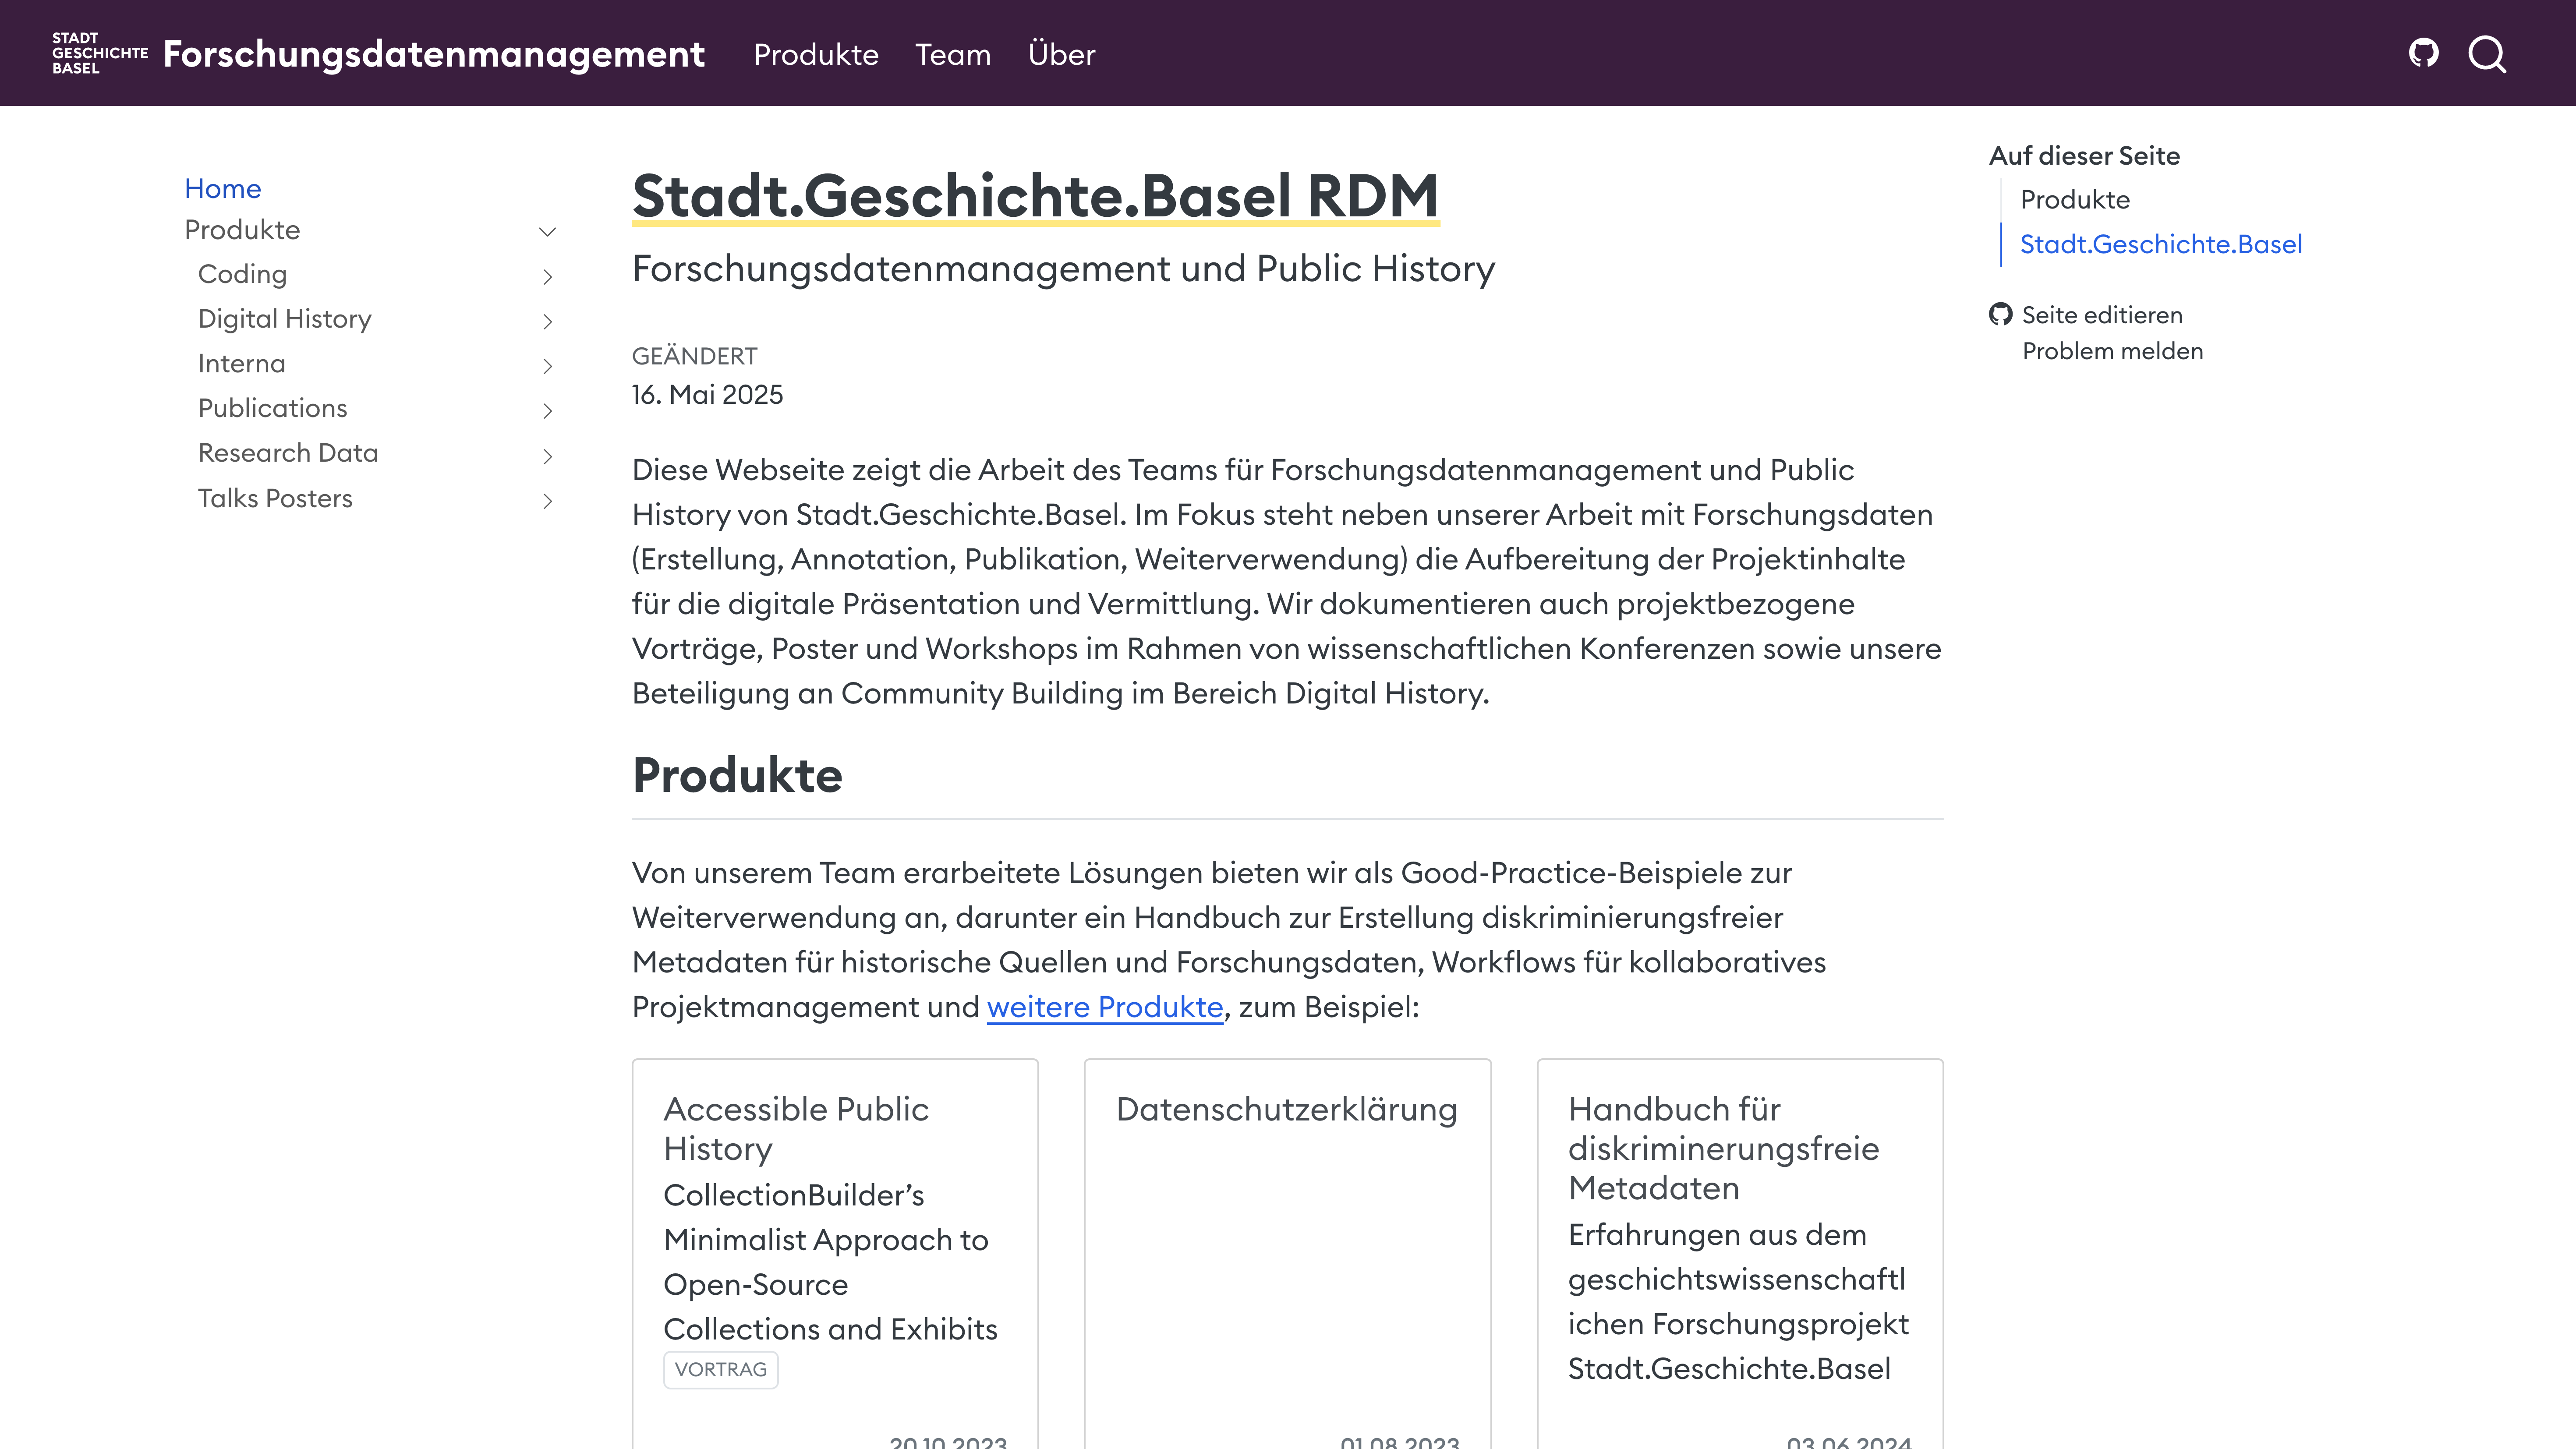
\includegraphics[width=0.9\linewidth]{images/dokumentation_stadtgeschichtebasel_ch.png}
  \caption{Website of \emph{Stadt.Geschichte.Basel RDM} presenting the team's work on research data management, public history, and examples of good-practice products such as guides, workflows, and talks.}
  \label{fig-sgb-rdm}
\end{figure}

For the Stadt.Geschichte.Basel project, we created a \href{https://forschung.stadtgeschichtebasel.ch/}{research data platform}~\cite{goerlich2023} to provide project-related, annotated research data, including dozens of scientific illustrations created with ggplot2 in R. The plots are made available on this platform, but we wanted to ensure access to the underlying R code as well. We could have uploaded the R code to the platform, but we did not want to push our less tech-savvy main audience (historians) away with uncontextualized source code, and we wanted the code to be 100\% reproducible. To publish the plots including a reproducible workflow -- from raw data to a PDF export of each plot -- we created the \href{https://dokumentation.stadtgeschichtebasel.ch/sgb-figures}{\textbf{sgb-figures}}~\cite{twente2025c} GitHub repository with our template. This repository provides a reproducible environment with raw data and scripts for processing, plotting, annotating, and exporting the available illustrations. Each plot is linked to from our research data platform. With the publication of our data and workflow, we make it possible for interested users to tweak parameters, add additional data, or reuse our dataset for other analyses.

\begin{figure}[t!]
  \centering
  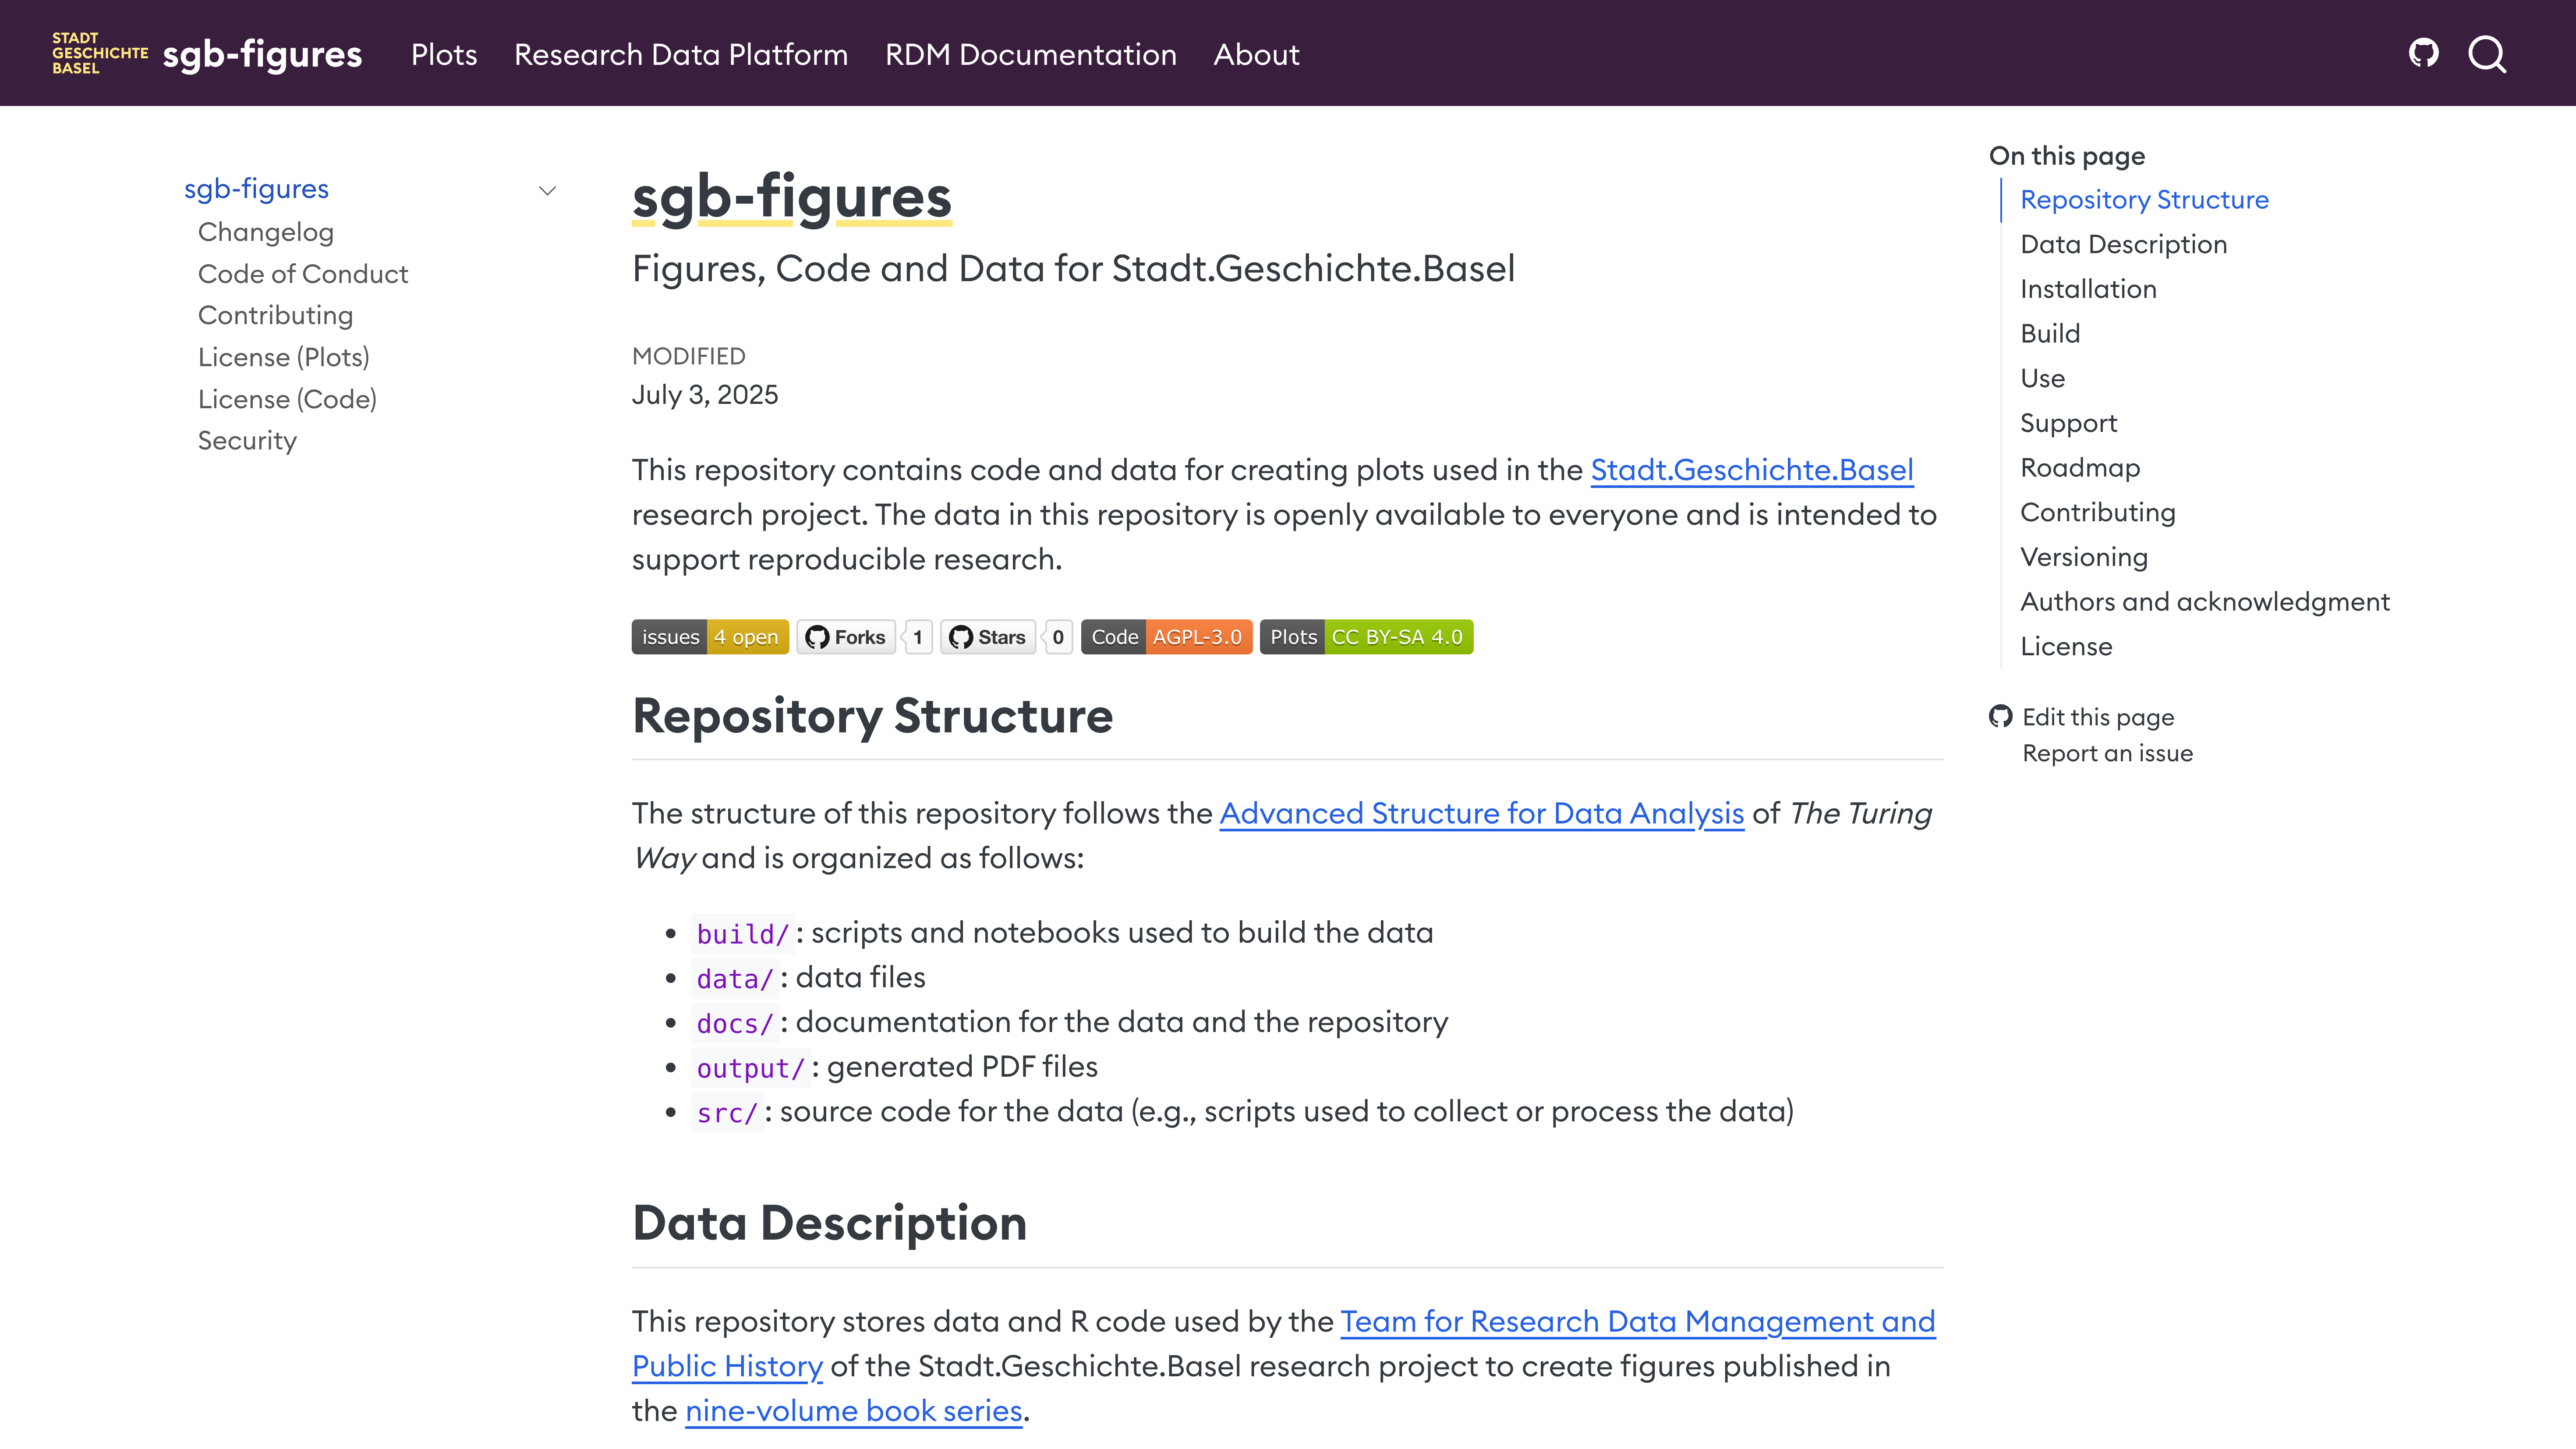
\includegraphics[width=0.9\linewidth]{images/dokumentation_stadtgeschichtebasel_ch_sgb_figures.png}
  \caption{Landing page of the \emph{sgb-figures} repository, presenting code, data, and documentation for creating plots used in the Stadt.Geschichte.Basel research project.}
  \label{fig-sgb-figures}
\end{figure}

\subsection{Reproducible Workflows}\label{reproducible-workflows}

A similar example is a repository containing voting data of members of the Danish Parliament, Folketing. The dataset itself is published in a GitHub repository at \href{http://mtwente.github.io/nordatlantisk-ft}{\textbf{mtwente.github.io/nordatlantisk-ft}}~\cite{twente2024a}, including the workflow to scrape the voting data from Folketinget's API, to combine different variables into one dataset, and to create a few exploratory visualizations. Using the template, we structured the repository according to best practices following an advanced structure recommended by \emph{The Turing Way}~\cite{theturingwaycommunity2025}, with a clear folder structure for raw data, processed data, analysis scripts, and documentation, including a codebook for all variables. The site also integrates external resources like a Zotero bibliography of relevant sources, demonstrating how contextual information can be linked to the dataset. The template's flexibility allows for including a short descriptive report on the data with self-updating, interactive plots as an integral part of the site, providing an initial overview of the data without having to delve into the data structure itself. The GitHub repository enables users to rerun the data scraping workflow themselves by making use of both R and GitHub features such as reproducible environments with R targets and Codespaces. Using GitHub Actions, the dataset can be updated at fixed time intervals -- including uploads to Zenodo -- without the need for manual intervention. By encapsulating this in the template, such maintenance tasks become standardized across projects.

\begin{figure}[t!]
  \centering
  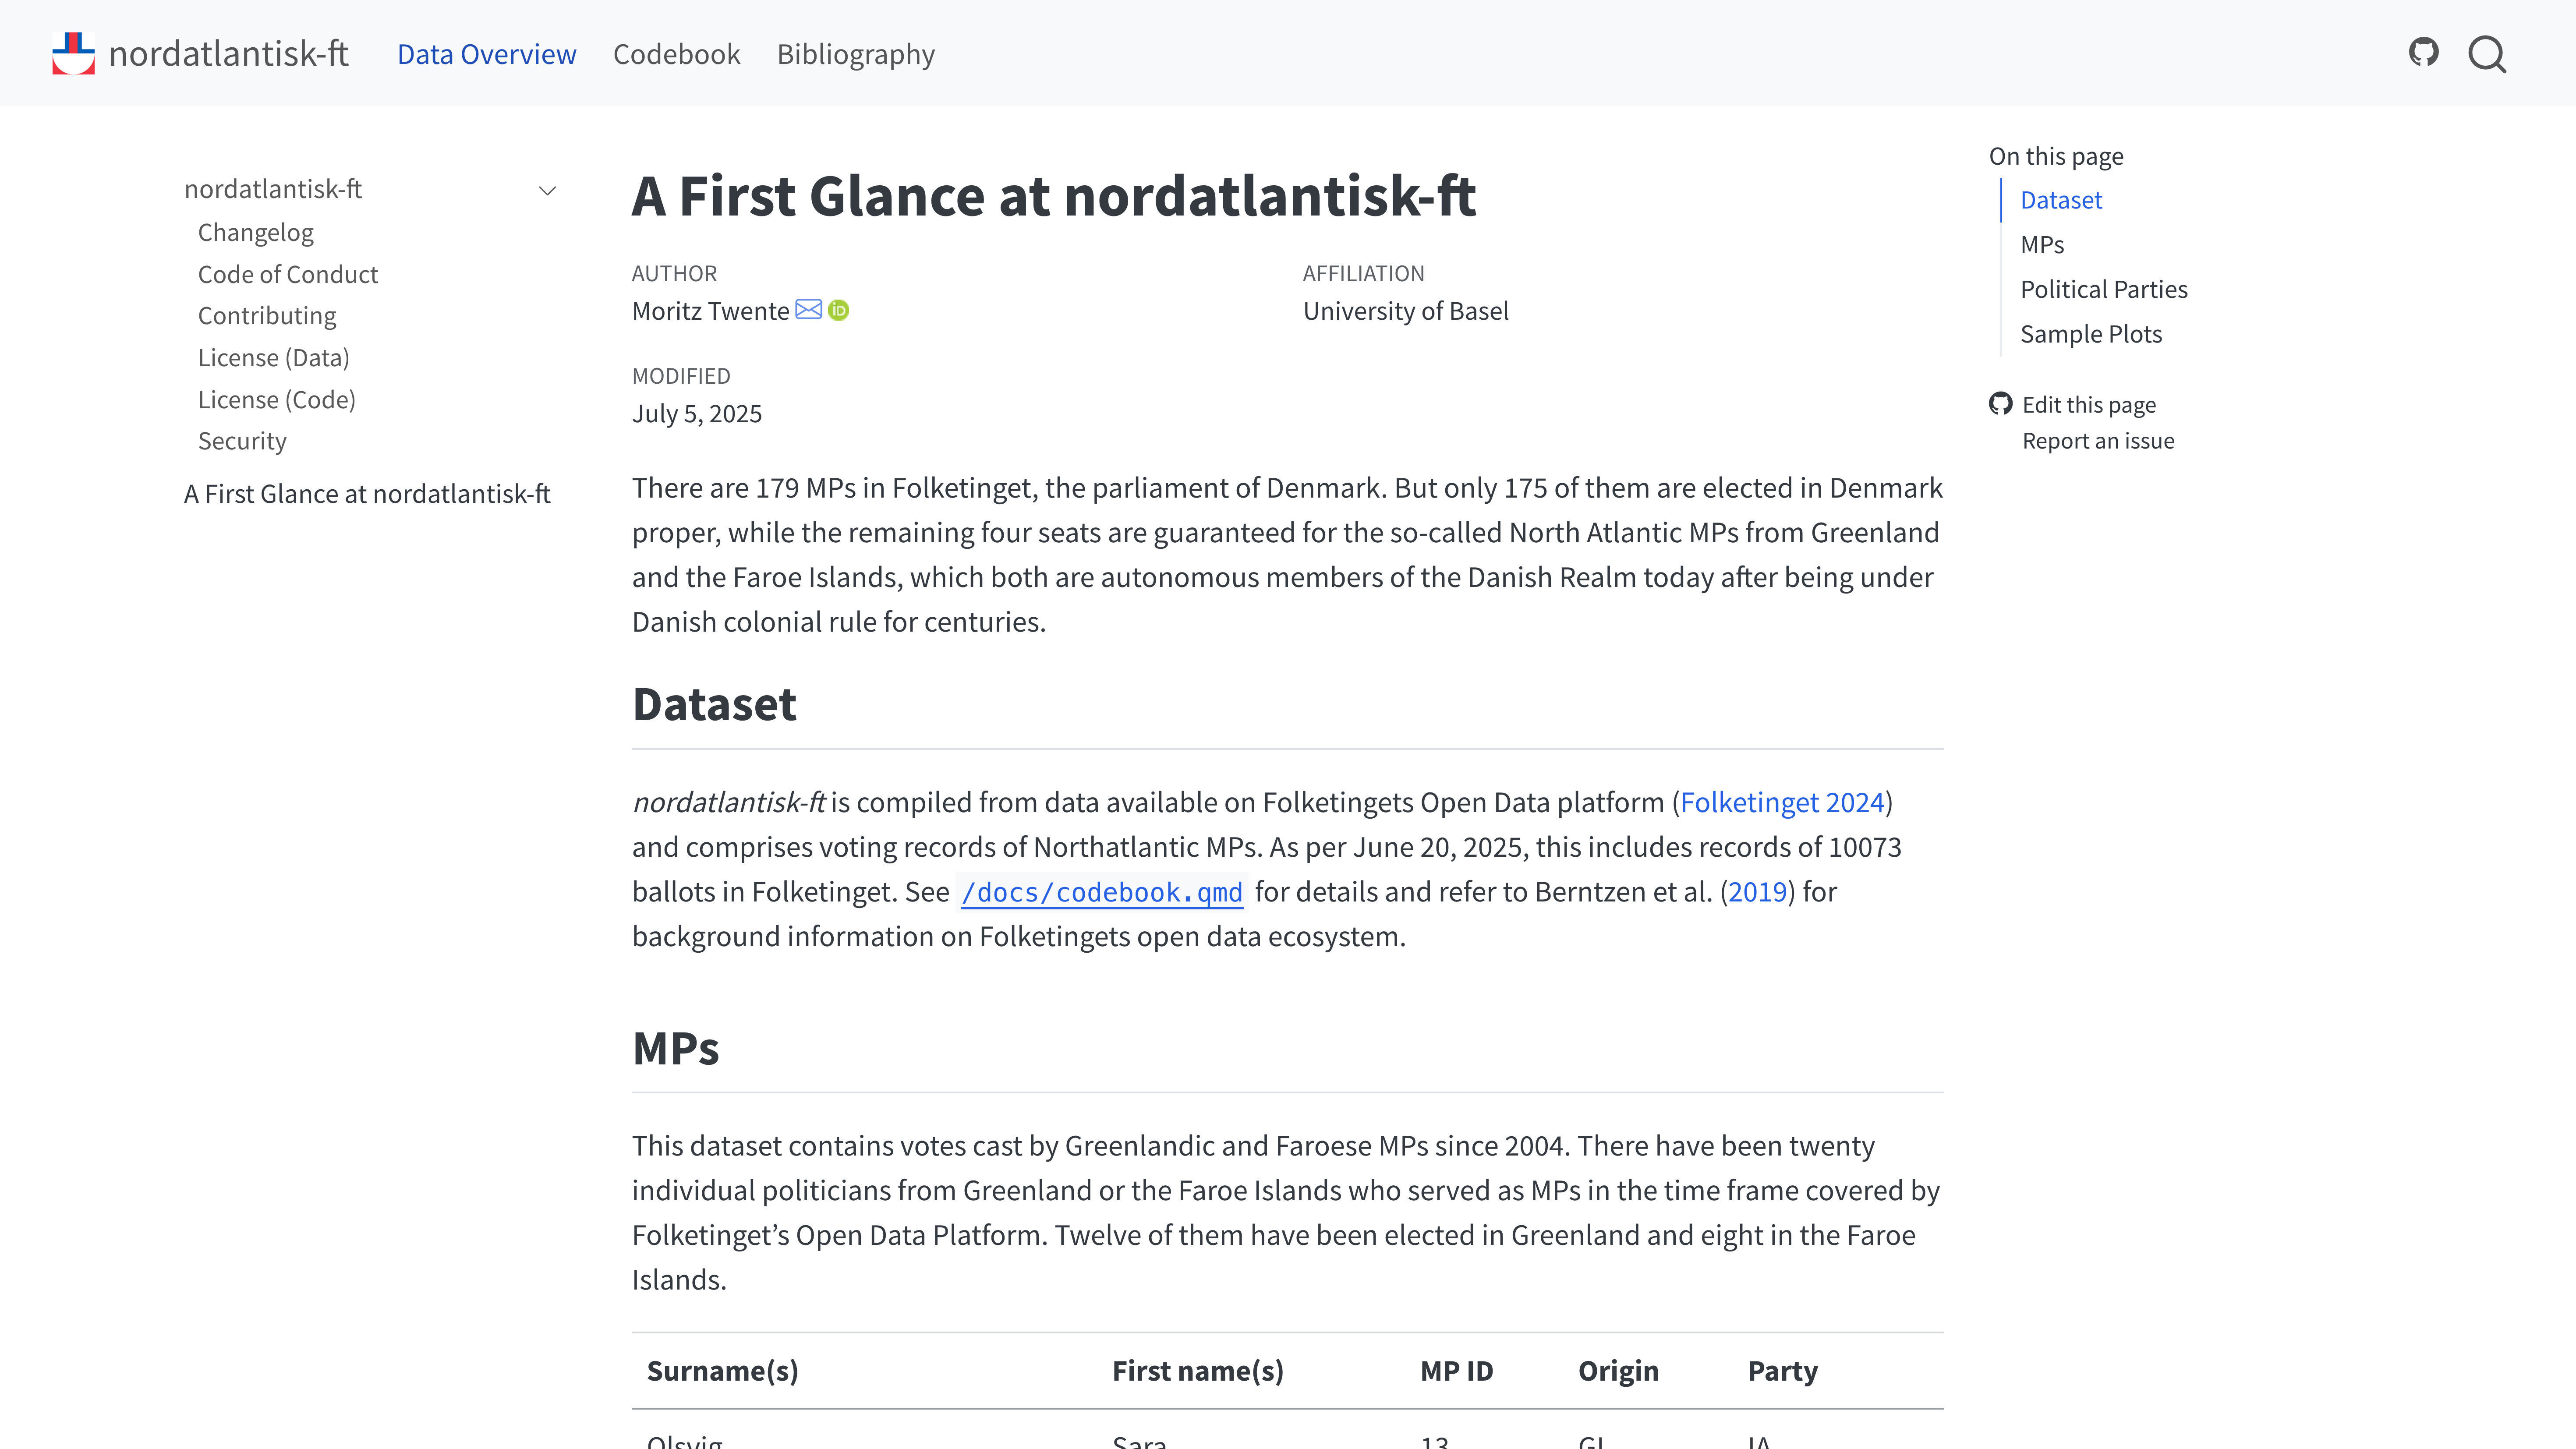
\includegraphics[width=0.9\linewidth]{images/nordatlantisk_ft_report.png}
  \caption{Landing page of the \emph{nordatlantisk-ft} project, presenting an overview of the dataset on North Atlantic MPs in the Danish parliament, including data sources and contextual information.}
  \label{fig-nordatlantisk}
\end{figure}

Even for projects that do not consist of one executable workflow, the template is useful for documenting which steps were taken to compile the research data to be published. Quarto's multi-language capabilities make it possible to document processing steps in written text, and, using flowcharts, also in a visually appealing way. Take the data repository \href{https://mtwente.github.io/maxvogt-analysis}{\textbf{maxvogt-analysis}}~\cite{twente2024} for example. In this project, spatial data and design attributes of railway station architecture in Switzerland were collected to conduct a study in urban design history. While photographs were archived on Wikimedia Commons, a separate location was needed to also store about fifty geojson files to provide results of urban morphology analyses. Using the Quarto template, it was not only possible to check the geodata into version control, but also to provide documentation on the data source and workflow in Markdown. A notable use of the template here was embedding a Mermaid.js diagram outlining the analysis workflow -- from data collection to analysis steps -- directly in the documentation. This diagram offers a quick visual understanding of how the research was conducted, complementing the textual description. By hosting the data and the Python analysis code together, the site becomes a one-stop resource for others interested in this approach to spatial analysis of architectural history. They can see the exact steps taken, map outputs, and even use the geodata in GIS or for interactive online maps using Leaflet.js.

\begin{figure}[t!]
  \centering
  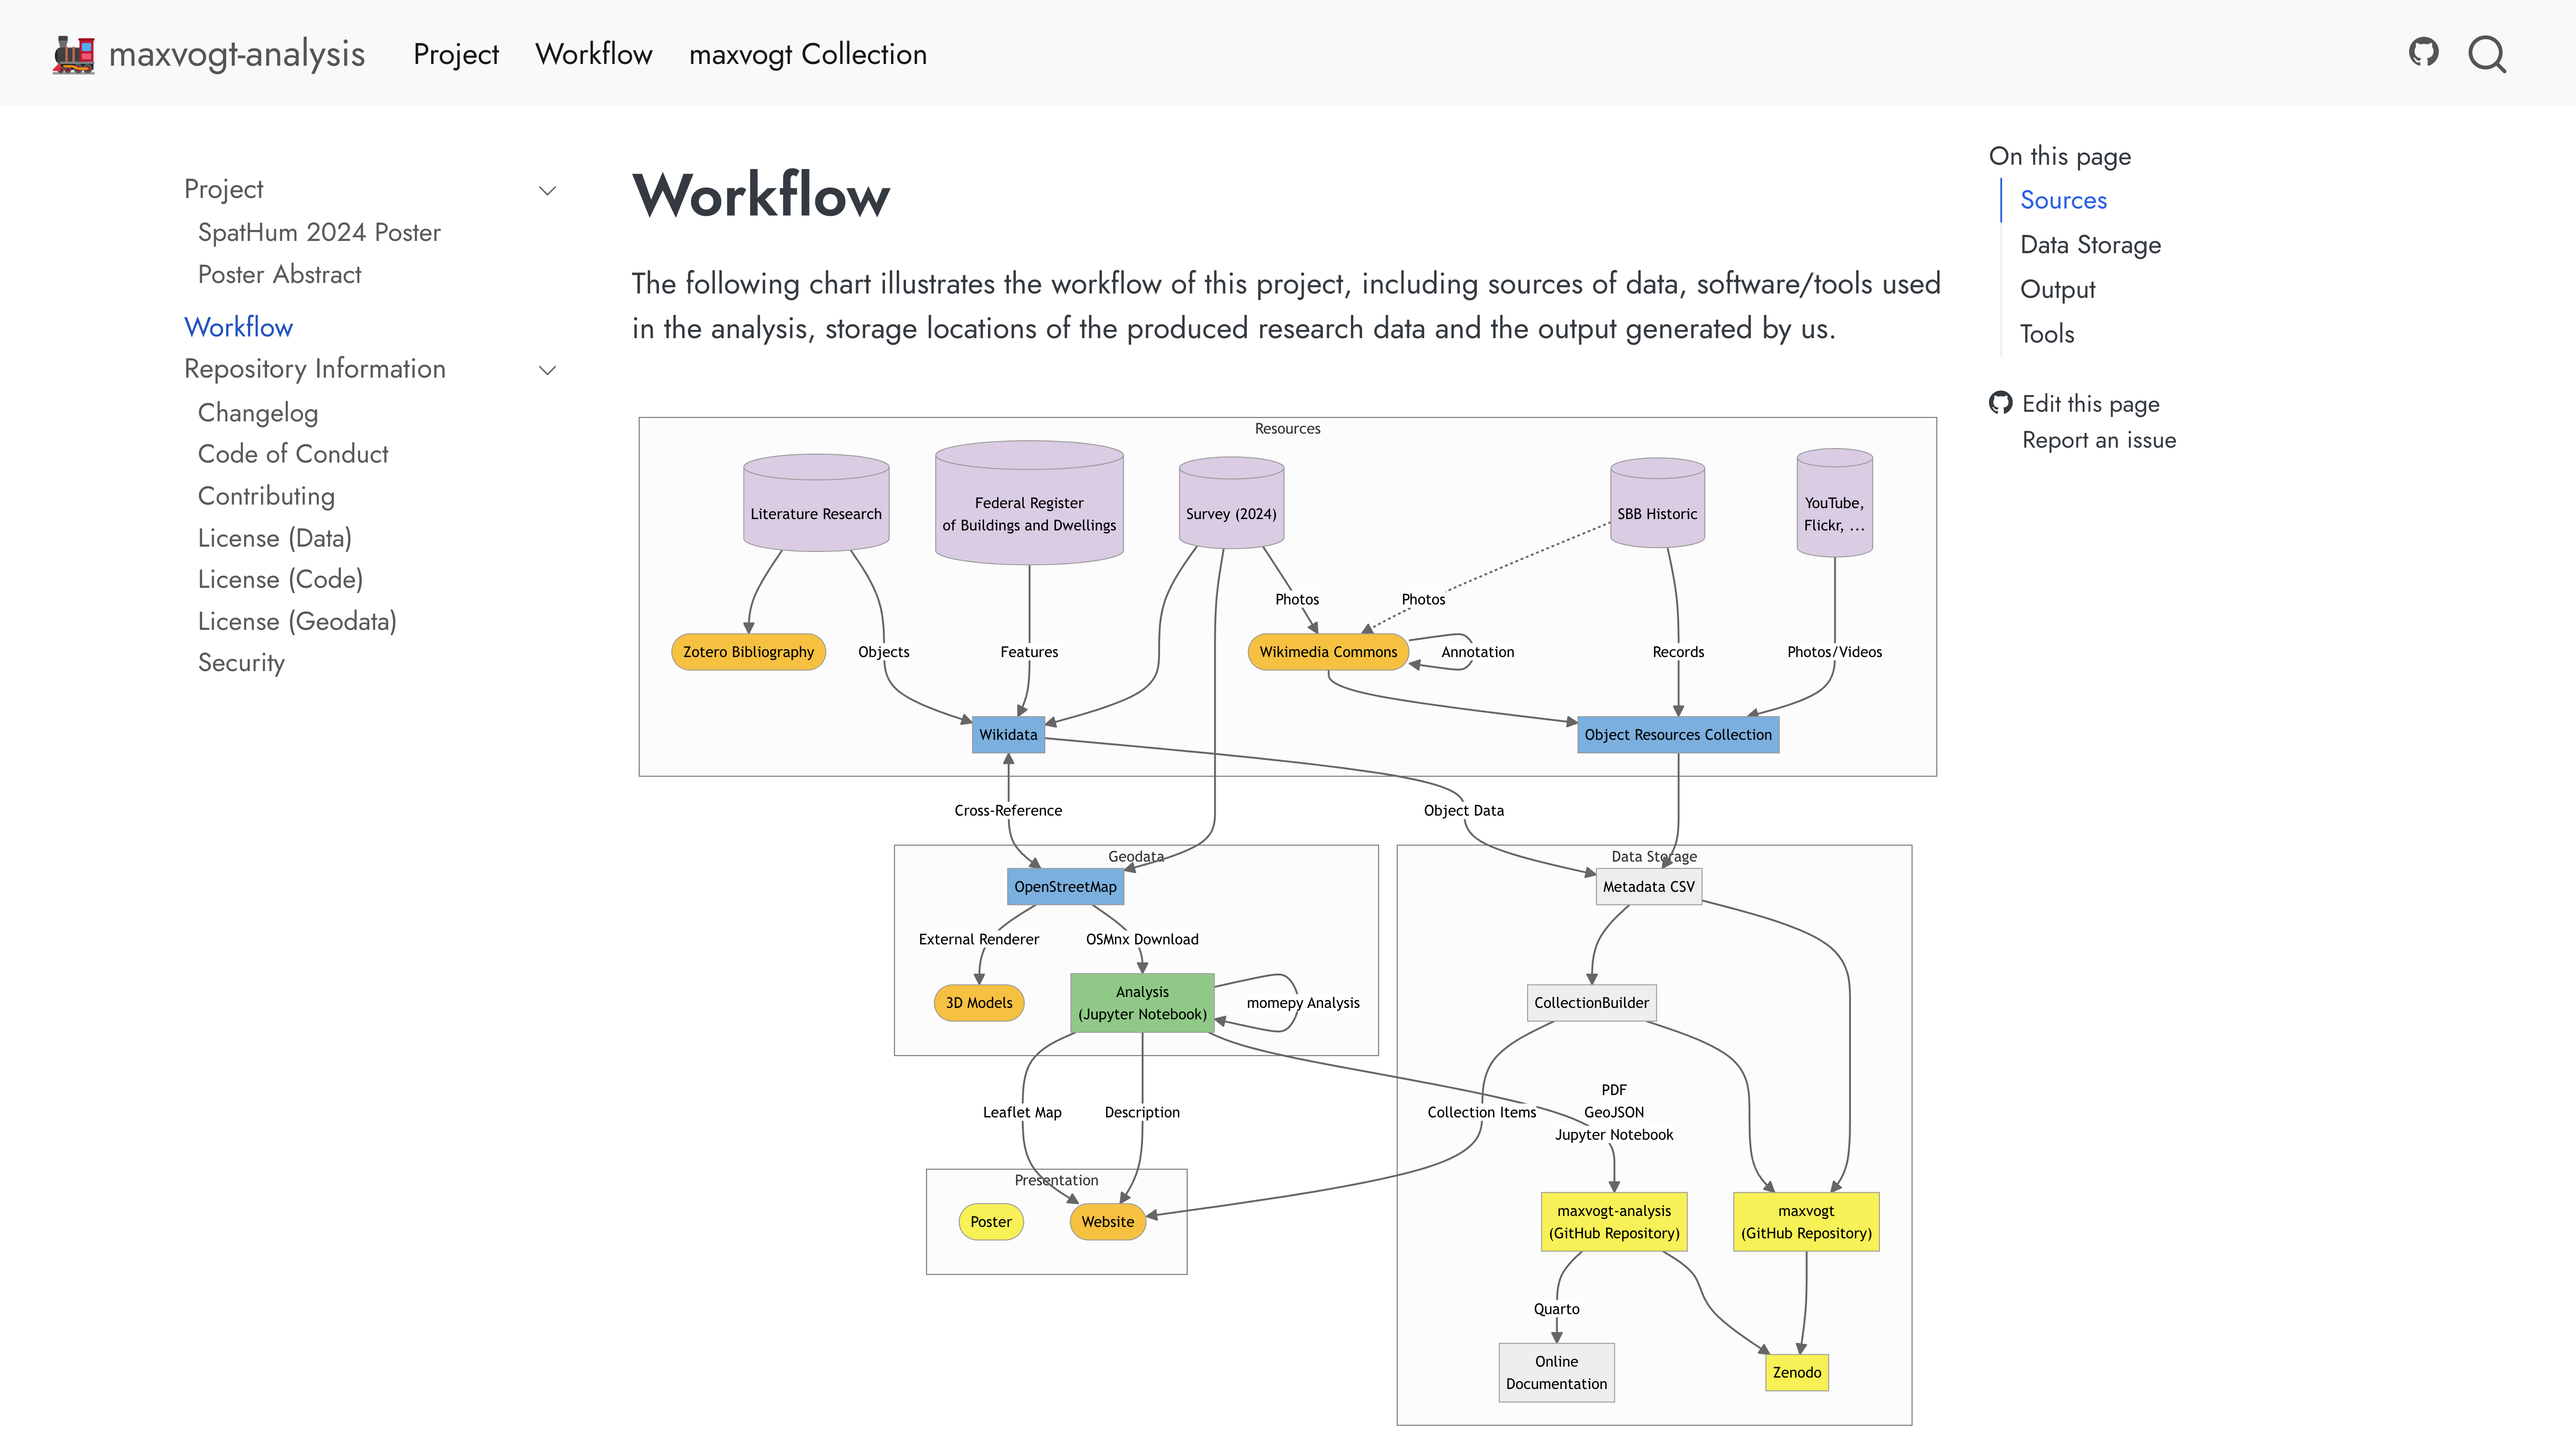
\includegraphics[width=0.9\linewidth]{images/maxvogt_analysis.png}
  \caption{Workflow diagram of the \emph{maxvogt-analysis} project, showing data sources, software tools, data storage, and resulting outputs.}
  \label{fig-max-vogt}
\end{figure}

The possibility to add multimedia content to the research data documentation is also part of the project \href{https://mtwente.github.io/modelling-marti}{\textbf{Modelling Marti}}~\cite{twente2025b} -- topic modeling for newspaper articles by Hans Marti, a pioneer of spatial planning in Switzerland. While the GitHub repository behind the Quarto website again stores the harvested data -- segmented text in txt and csv files, including metadata -- it allows for a publication focused on narrative elements and context as well. The site reads like an extended article: It lays out the research questions, methods (article scraping, data cleaning, topic modeling), and the results with exploratory charts and tables. However, unlike a traditional paper, it includes the underlying code for topic modeling or word frequency analysis inline using R, which readers can inspect or even replicate with tweaked parameters. By employing the template, we turned what could have been a static PDF into an interactive publication. Interactive maps using Leaflet.js and historic photographs embedded from ETH Zürich's \href{https://e-pics3.ethz.ch/de/home/}{e-pics catalogue} enhance the reading experience by turning the data repository into a narrative, data-driven publication. It also serves as a proof of concept that academic publications in history can be made more transparent and reproducible without sacrificing narrative clarity.

\begin{figure}[t!]
  \centering
  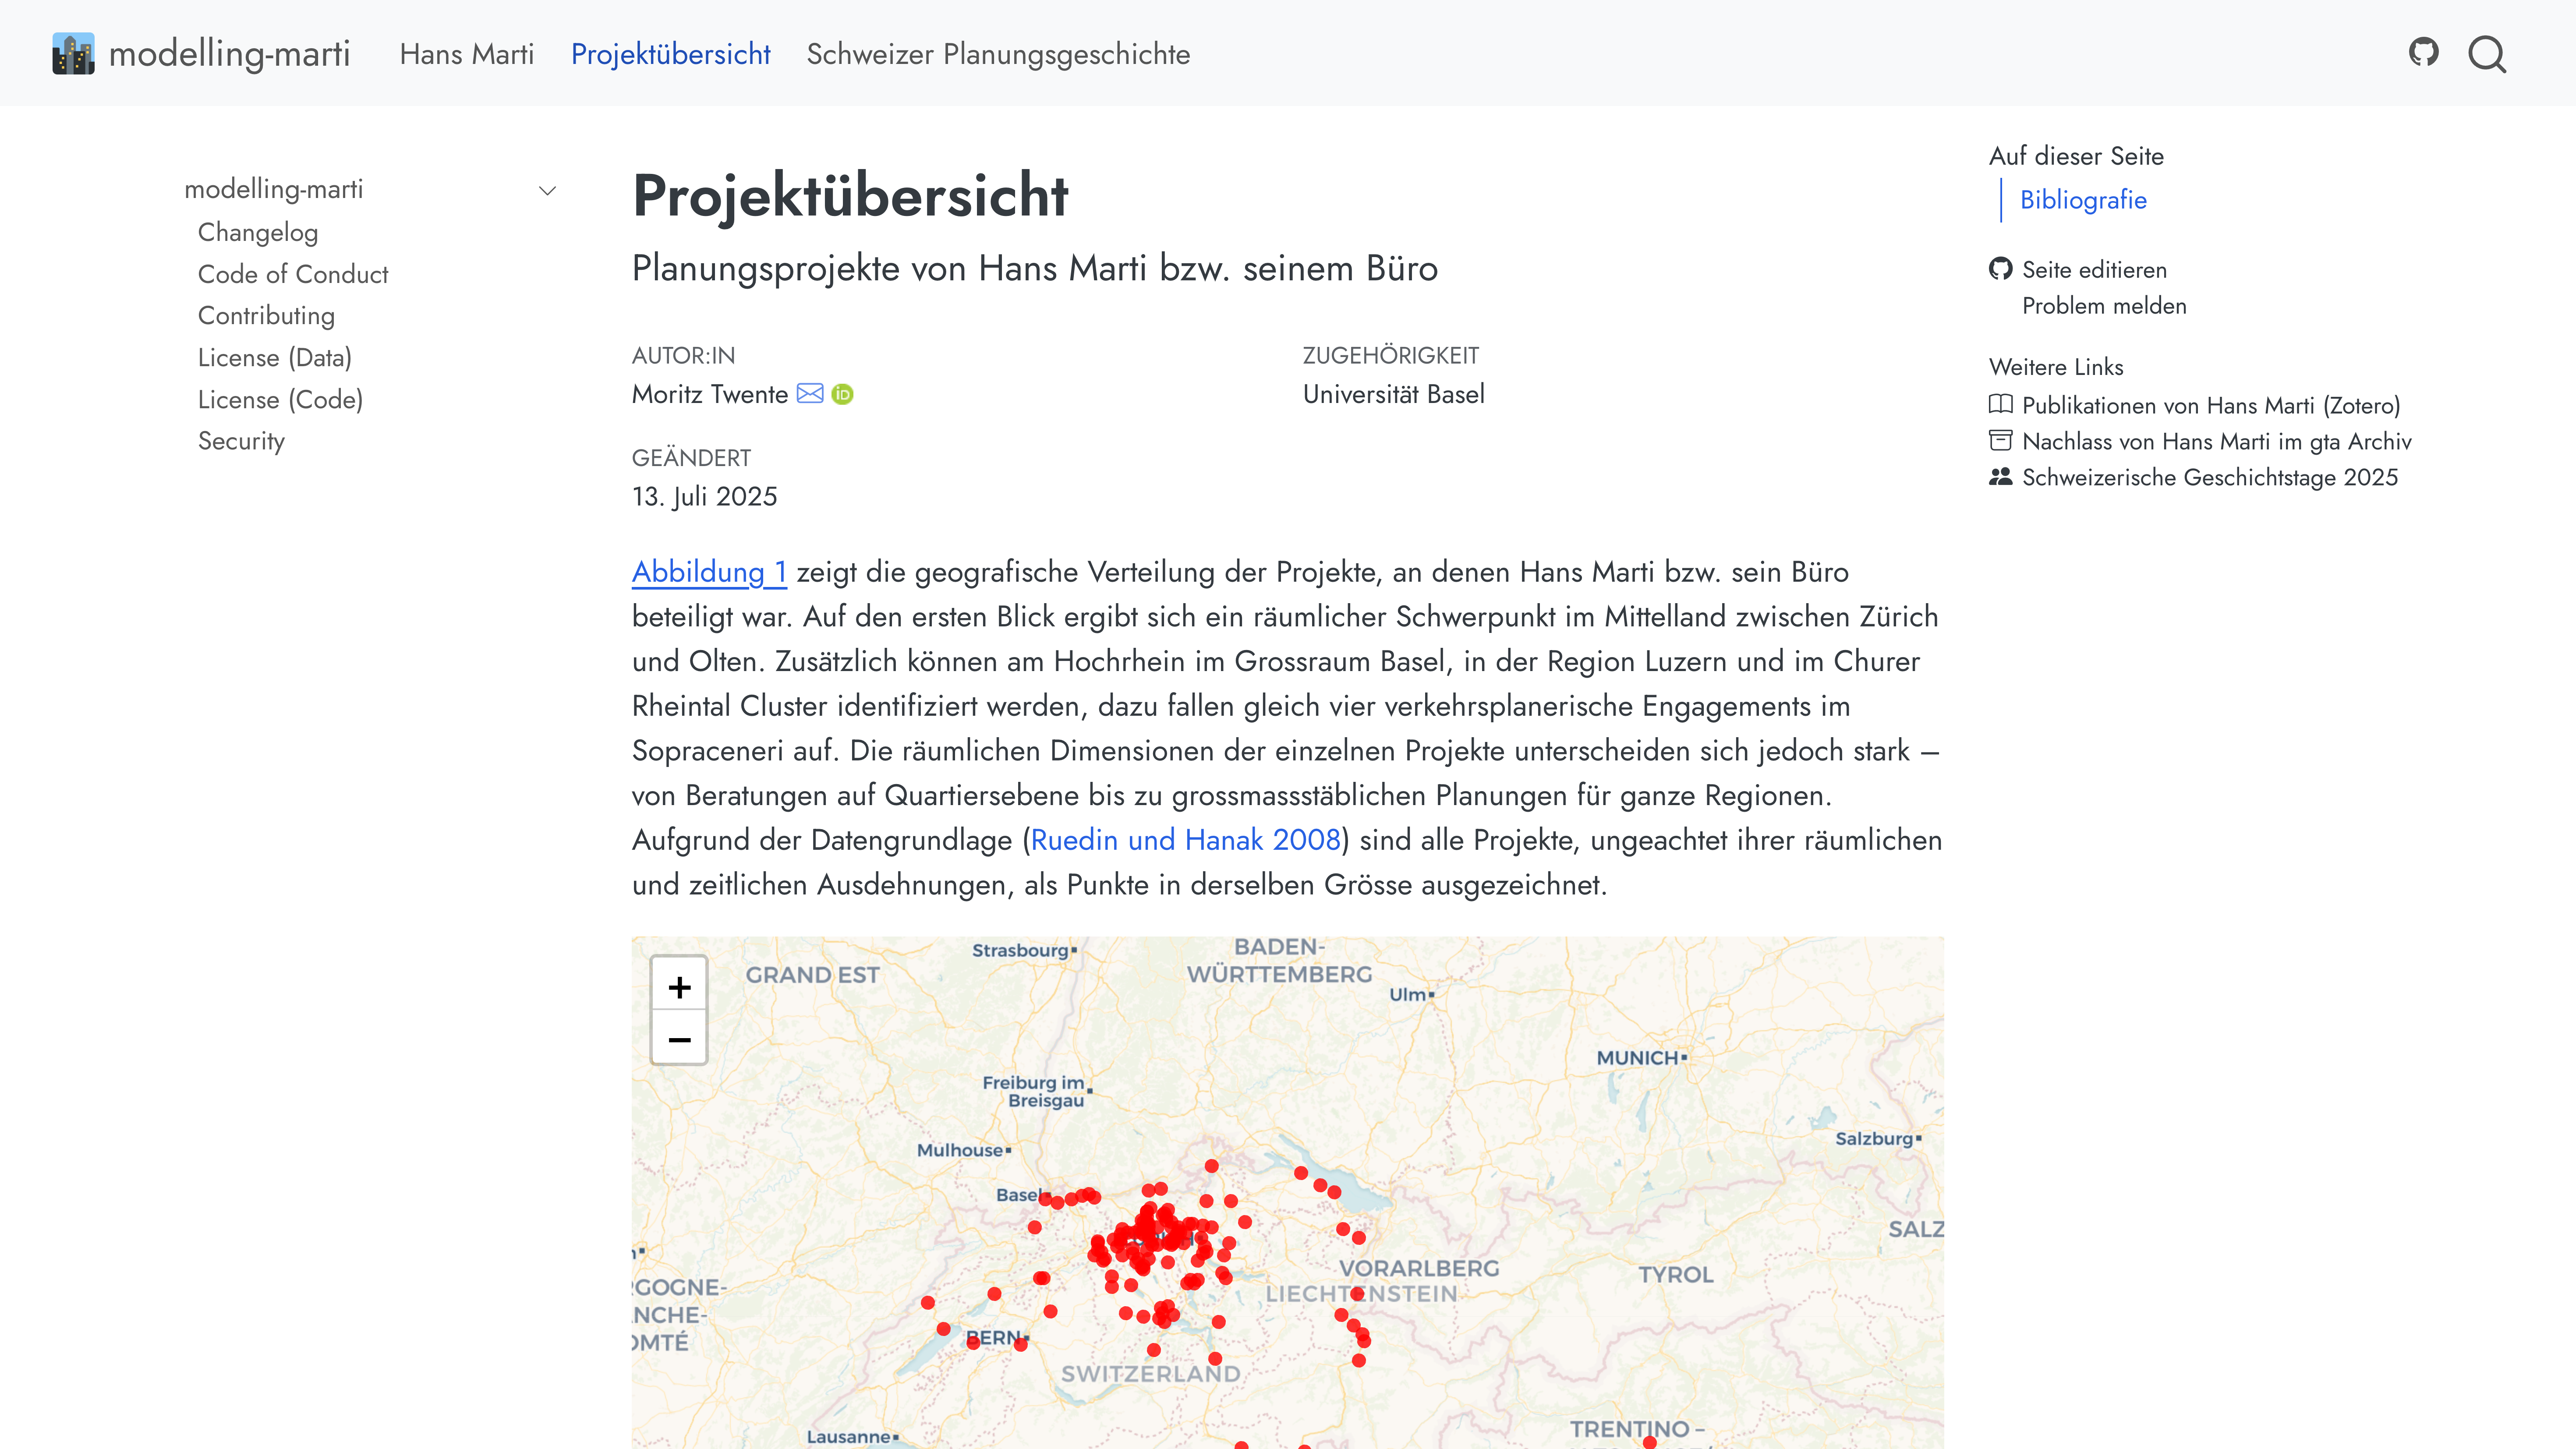
\includegraphics[width=0.9\linewidth]{images/modelling_marti.png}
  \caption{Overview page of the \emph{modelling-marti} project, presenting planning projects by Hans Marti and his office, including a map of their geographic distribution.}
  \label{fig-modelling-marti}
\end{figure}

\subsection{Conference and Teaching Platforms}\label{conference-and-teaching-platforms}

The Open Research Data Template has proven useful beyond traditional research data documentation -- notably in academic event and course contexts. We deployed the template for the \href{https://digihistch24.github.io/}{\textbf{Digital History Switzerland 2024 conference}}~\cite{baudry2024b}. Here, the template was used to publish the \emph{book of abstracts}~\cite{baudry2024a} as an interactive digital publication. Each abstract is a short, citable publication with references, some accompanied by dynamically generated visualizations. The site not only provided information to conference attendees but also now serves as a preserved record of the event, with DOIs ensuring each abstract is citable and archived using Zenodo. By using our template, we ensured that the process of compiling, formatting, and publishing the abstracts was largely automated and consistent, enabling researchers unfamiliar with Quarto and markdown to contribute to the book of abstracts. Thanks to the template, we are also independent of the university's conference management tools, which are not designed to be long-term archivable. Presenters submitted their abstracts (some with code snippets, bibliography files, or data links) as Markdown, which we integrated into the Quarto-based site. The inclusion of executable snippets allowed presenters in computational history to share live examples alongside their abstract text, something not possible in a static PDF. This use case demonstrated that the template can handle multi-author content and still maintain overall cohesion and quality control via versioning and automated checks.

\begin{figure}[t!]
  \centering
  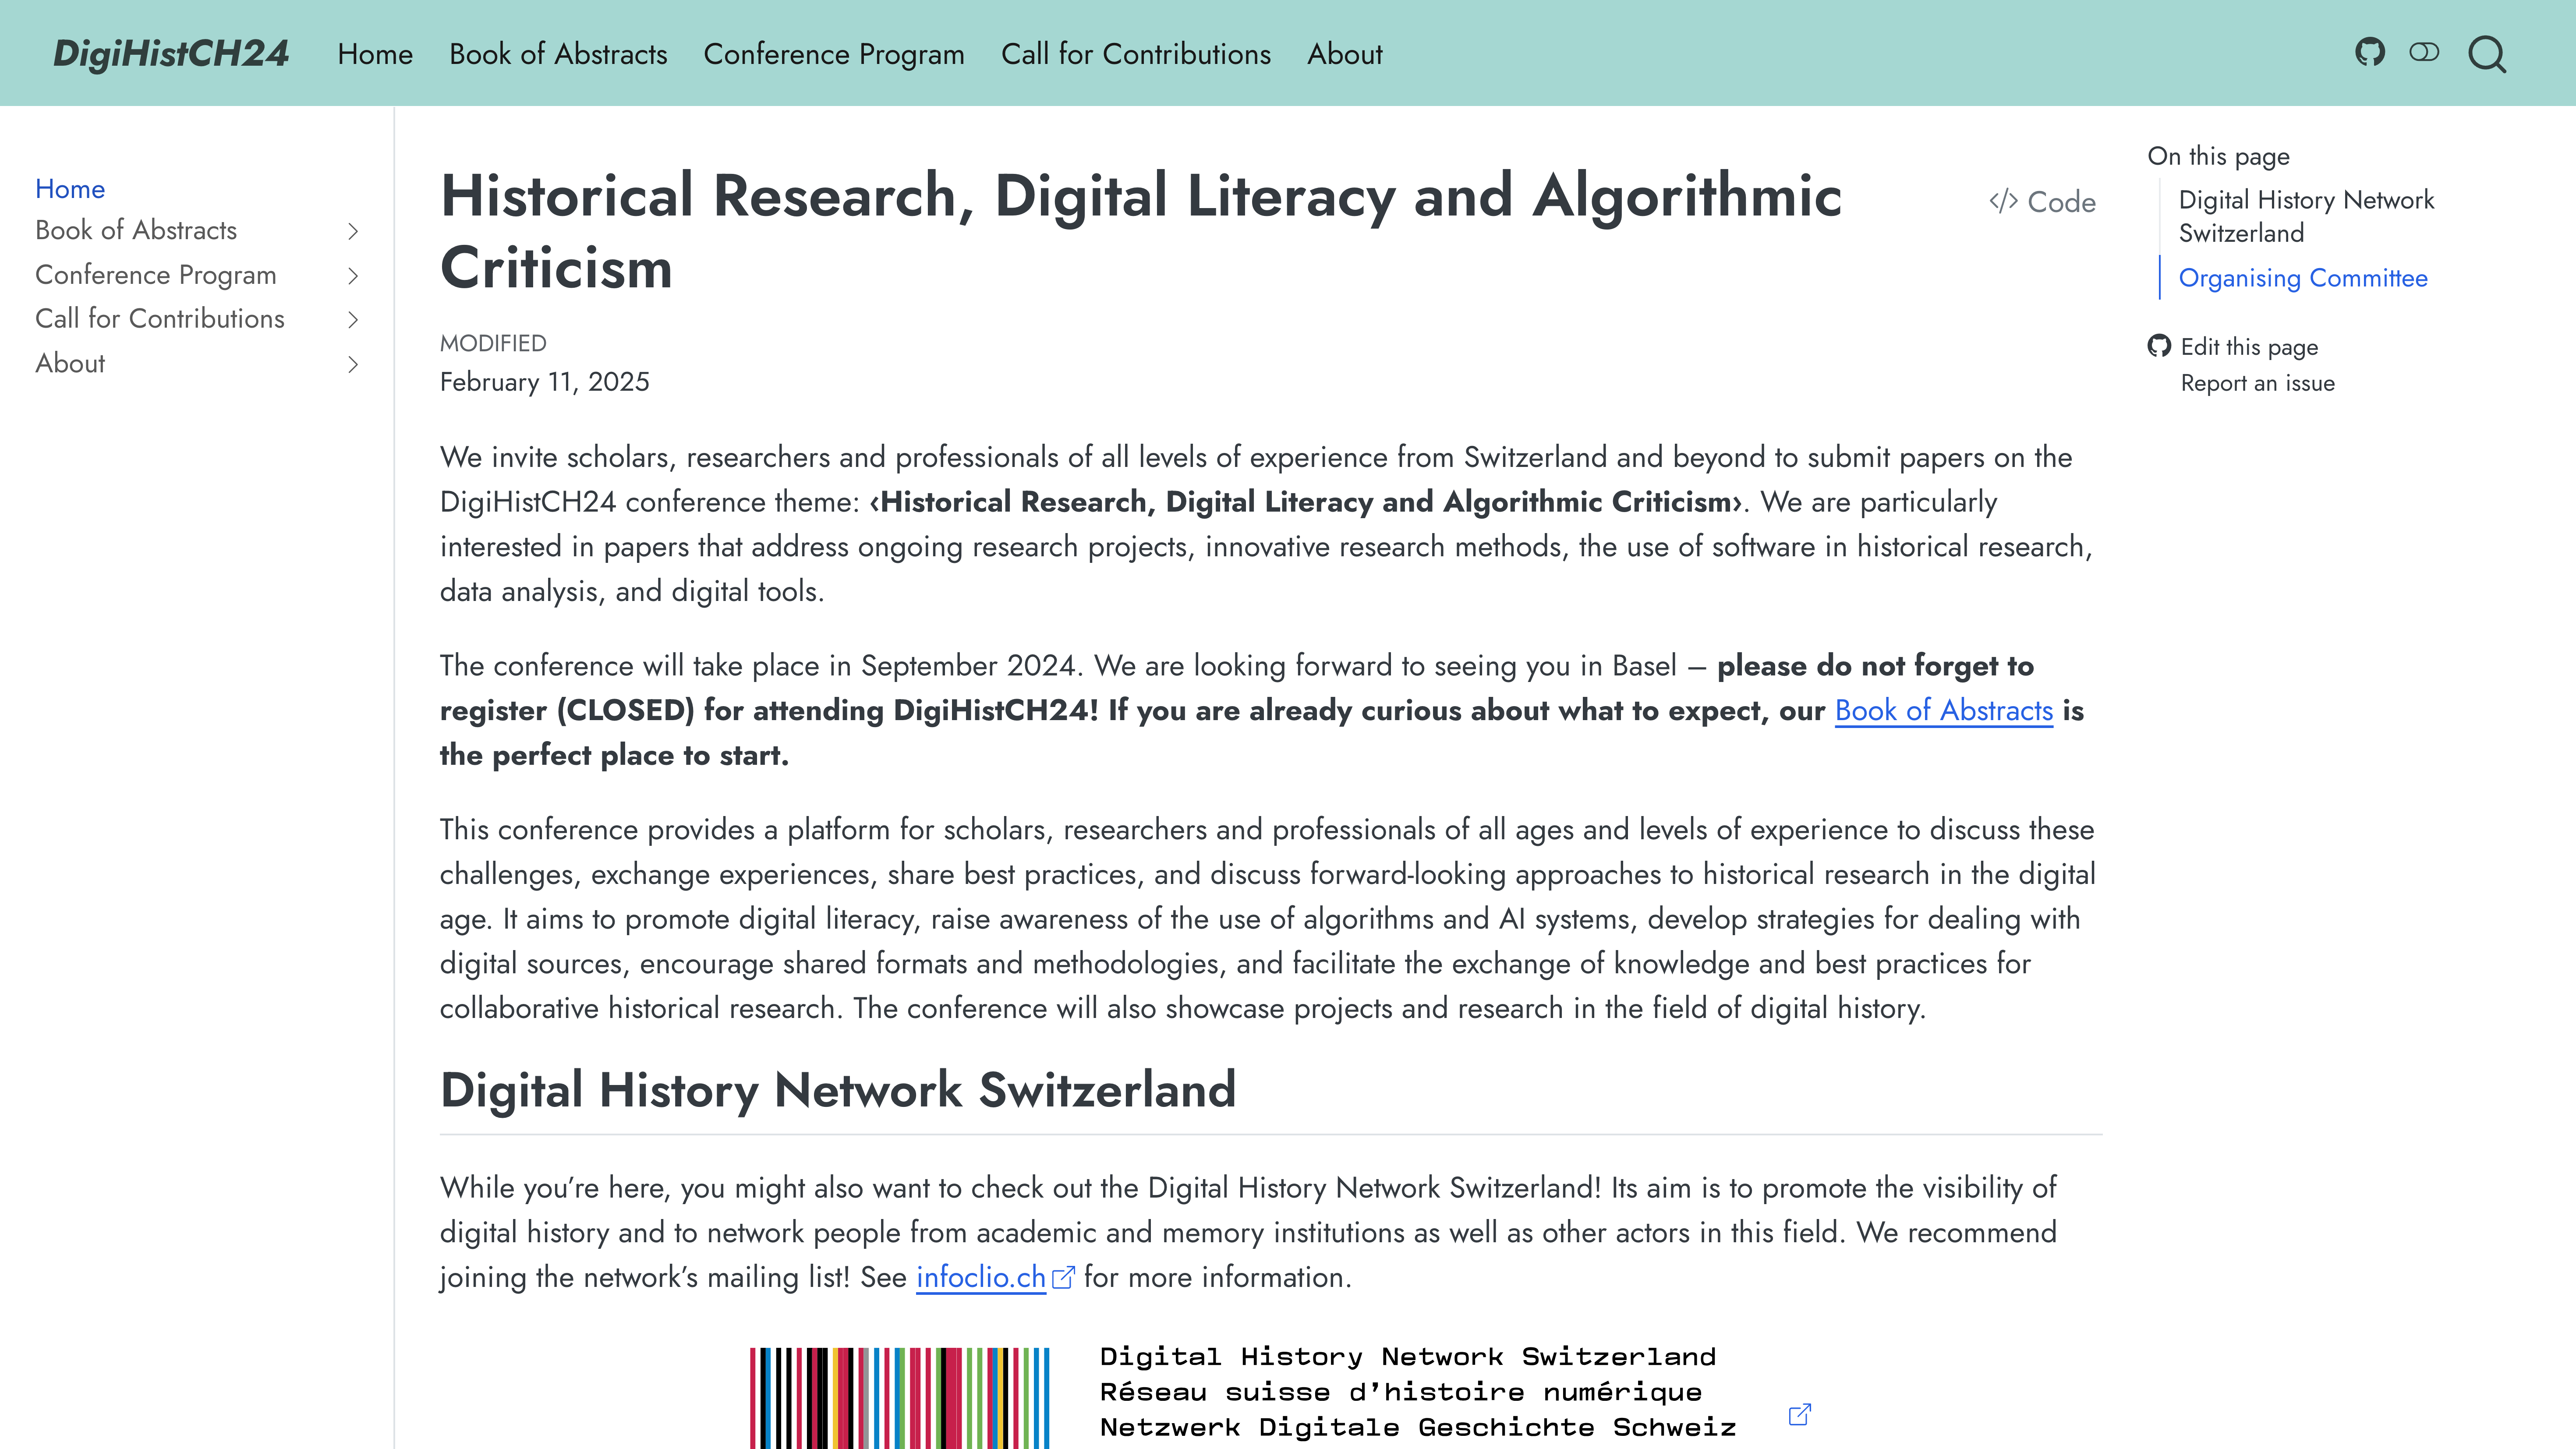
\includegraphics[width=0.9\linewidth]{images/digihistch24.png}
  \caption{Landing page of the DigiHistCH24 conference, introducing the theme ``Historical Research, Digital Literacy and Algorithmic Criticism'' and inviting participation.}
  \label{fig-digihist24}
\end{figure}

In a different vein, the \href{https://dhbern.github.io/}{\textbf{Digital Humanities Bern (DH Bern) website}}~\cite{digitalhumanitiesbern2025} was created with the template to serve as a hub for the University of Bern's DH projects and activities. Unlike the focused research cases above, this website aggregates various content types: blog posts, project descriptions, and event announcements. The template's flexibility allowed us to support all these content types within one site. For example, the portal features an events calendar (fed by data that can be updated via a simple CSV or Google Sheets and then pulled into the site), and a blog where each post can include interactive elements (one post visualized the timeline of DH projects at the university using an embedded chart). By building the site on the template, the DH Bern team benefits from the same maintainability -- any content update triggers a site rebuild, and the site's static hosting means it is low maintenance. Additionally, the portal harmonizes multiple projects and methodologies under a single framework. For instance, if one project is an online database and another is a mapping tool, their documentation on the portal can both use interactive code cells to show usage examples, providing a unified user experience. The success of this portal indicates that our template can double as a general-purpose static site generator for academic groups, not just data-specific projects.

\begin{figure}[t!]
  \centering
  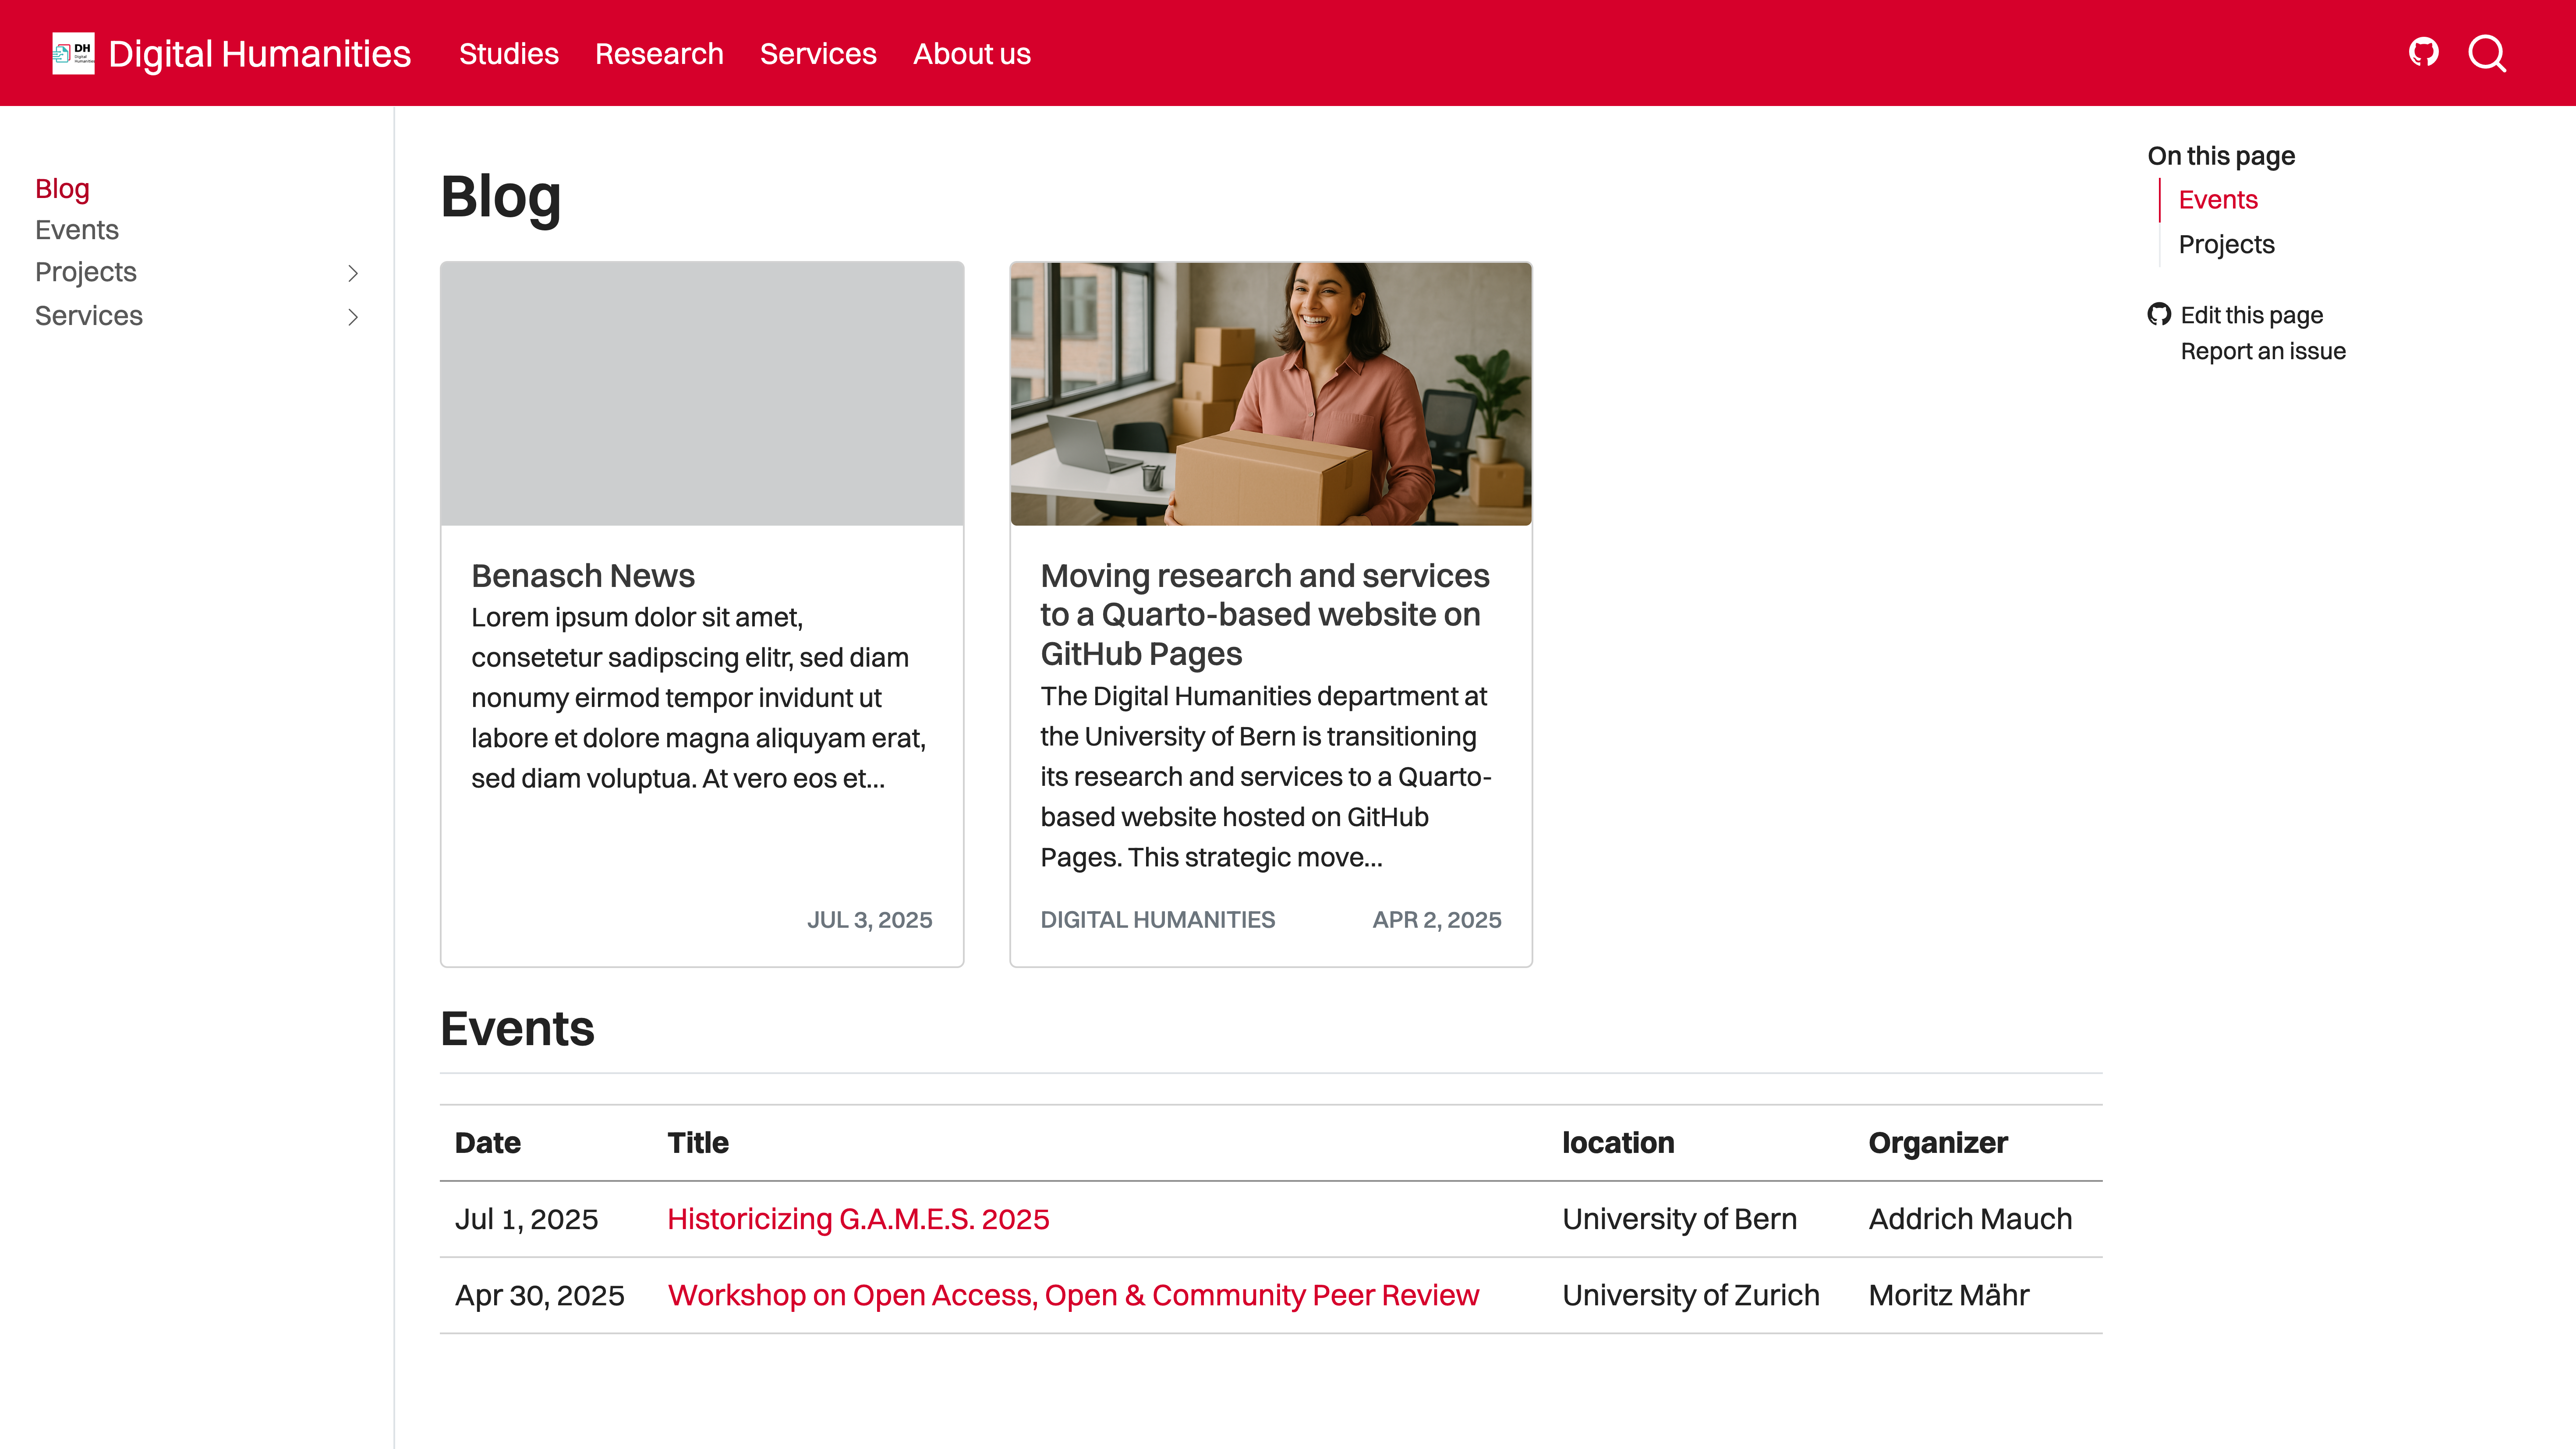
\includegraphics[width=0.9\linewidth]{images/dhbern.png}
  \caption{Blog and events page of the Digital Humanities department at the University of Bern, featuring news updates and upcoming events.}
  \label{fig-dh-bern}
\end{figure}

We also created a course website for \href{https://dhbern.github.io/decoding-inequality-2025/}{\textbf{Decoding Inequality}}~\cite{huber2024}, a university course by Rachel Huber and Moritz Mähr taught at the University of Bern for Digital Humanities students in 2025, using the template. This site hosted lecture notes, datasets for student exercises, and an interactive bibliography on machine learning and social inequality. Moreover, the contributions of the students were uploaded as well, turning the site into a collaborative space. The static nature of the deployed site meant that it was reliable and fast for students to access, and after the course ended, it remains a publicly accessible resource.

\begin{figure}[t!]
  \centering
  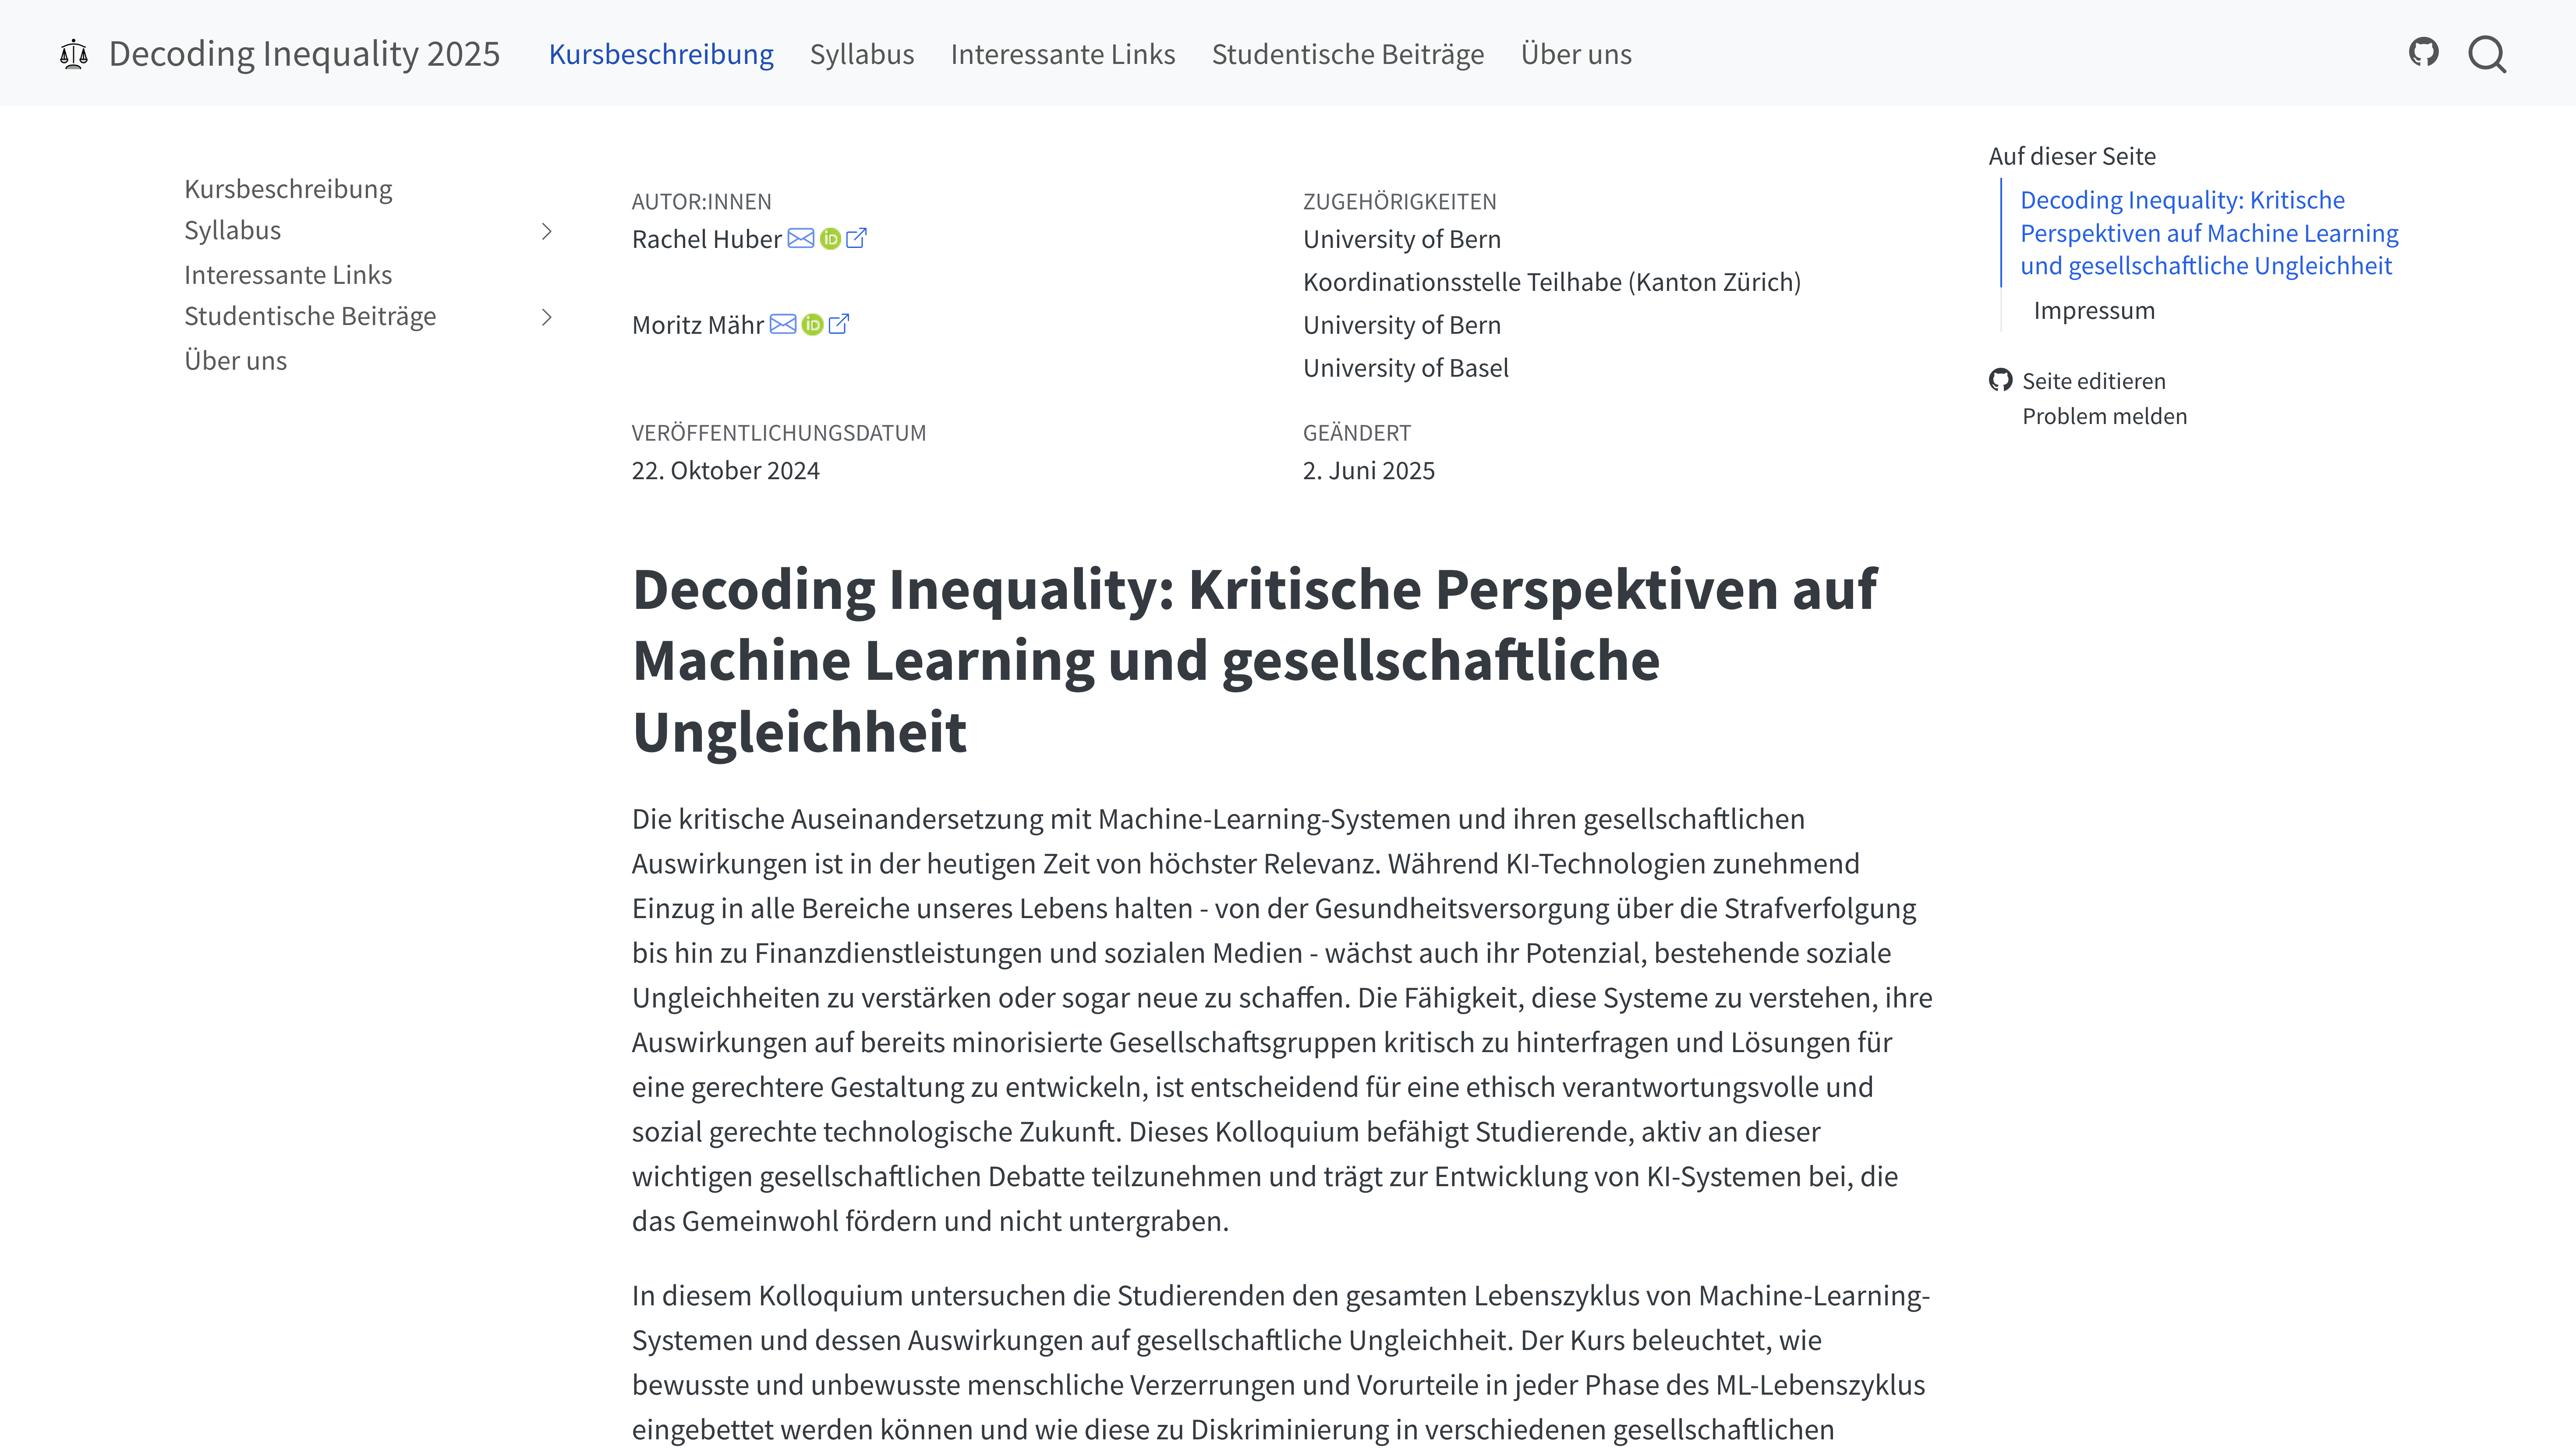
\includegraphics[width=0.9\linewidth]{images/decoding_inequality_2025.png}
  \caption{Course description page for \emph{Decoding Inequality 2025}, outlining the seminar's critical approach to machine learning systems and their societal impacts.}
  \label{fig-decoding-inequality}
\end{figure}

\subsection{Living Publications and Handbooks}\label{living-publications-and-handbooks}

One of the most significant outcomes of our work has been the creation of a ``living handbook'' on \href{https://maehr.github.io/diskriminierungsfreie-metadaten/}{\textbf{Non-discriminatory Metadata}}~\cite{maehr2024d} for historical collections. This handbook, published in 2024 by Noëlle Schnegg and Moritz Mähr, was built using the template and exemplifies how scholarly documents can remain dynamic. The handbook provides guidelines and case studies on creating inclusive, non-discriminatory metadata in cultural heritage and research contexts. Because it is built with our template, it is not a static PDF but a multiformat publication that can continuously evolve -- indeed, it is explicitly intended as a ``Living Document'' open to continuous community development. The site allows readers to not only read the guidelines but also see examples of metadata records, some of which are interactive (e.g., forms or JSON examples that users can toggle). We included a discussion forum via the GitHub issues integration, inviting feedback or contributions from librarians, archivists, and others in the community. Notably, we took advantage of Quarto's multi-format output capabilities to release the handbook in multiple formats from the same source: an HTML website, a downloadable PDF, and even a Word document for those who prefer or require that format. All these formats are generated automatically, ensuring consistency across them. The template's DOI integration was used to archive a version of the handbook on Zenodo at the time of official release, giving it a citable reference. However, the online version continues to be updated with new examples and clarifications as the field evolves. This use case underlines how the template supports sustainability and accessibility: by making the handbook a static site, it remains accessible long-term (no dependency on a complex database or CMS), and by archiving versions, we balance the living nature with scholarly referenceability.

\begin{figure}[t!]
  \centering
  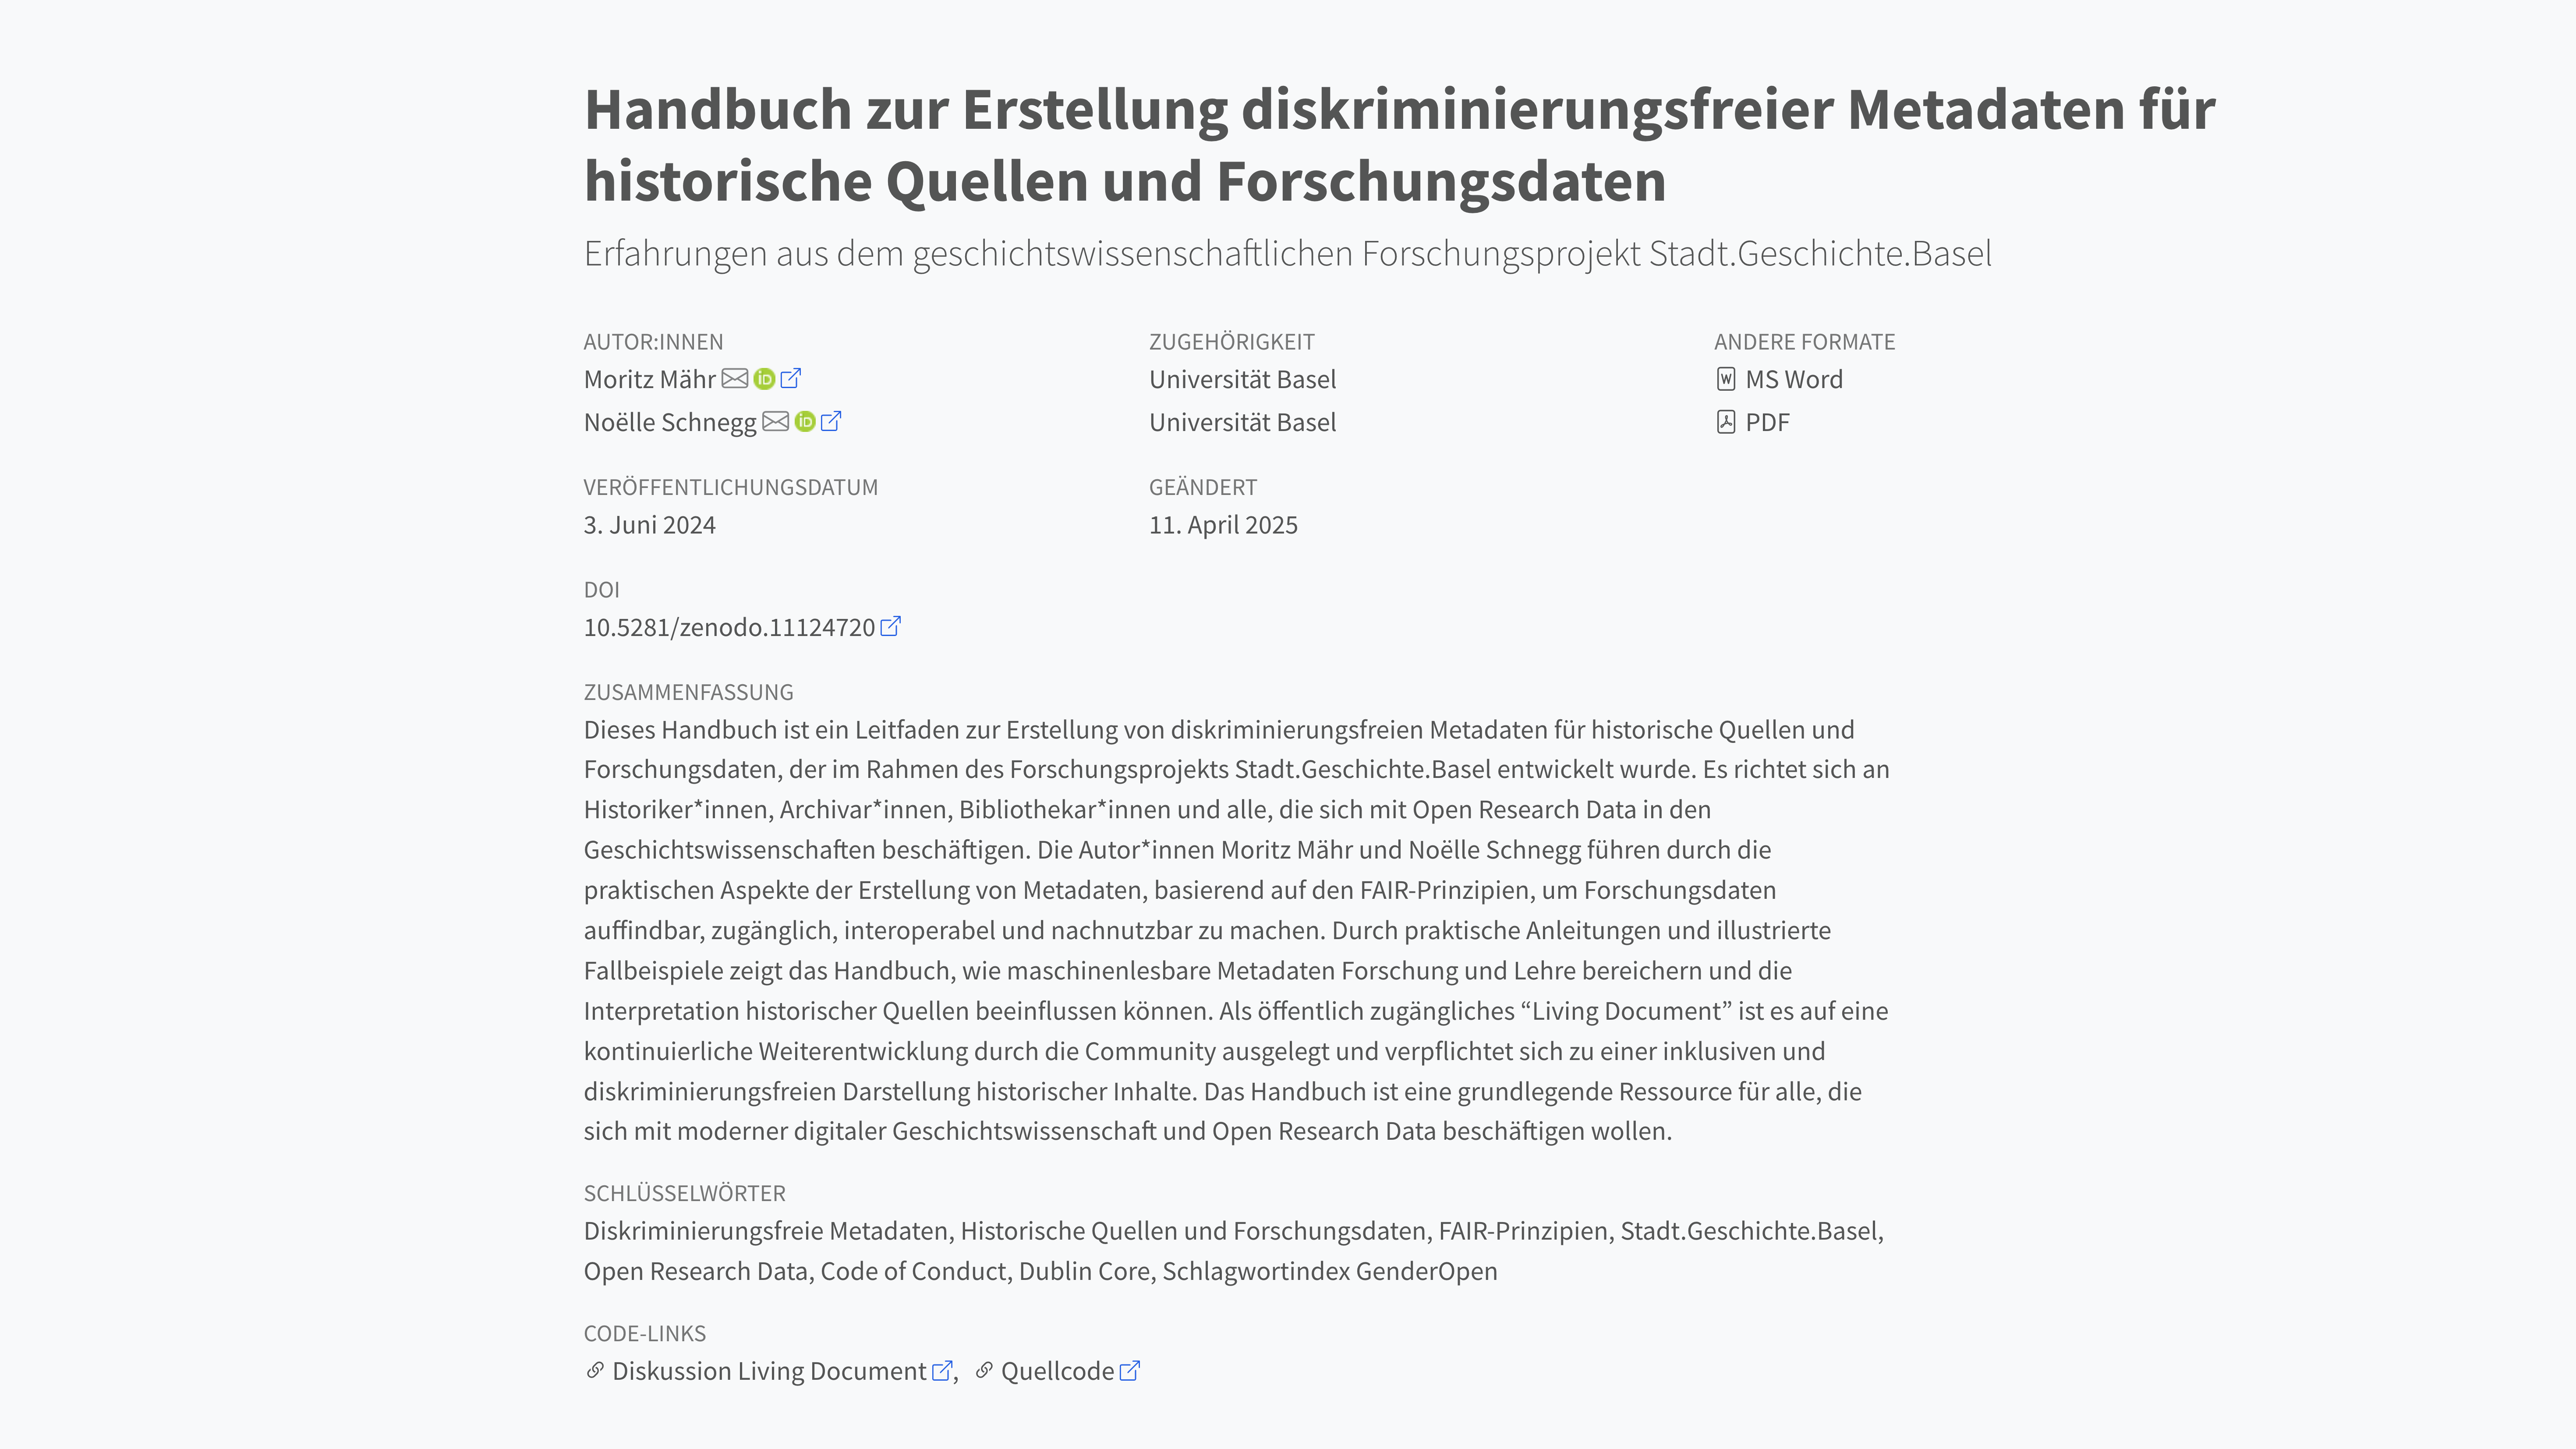
\includegraphics[width=0.9\linewidth]{images/diskriminierungsfreie_metadaten.png}
  \caption{Handbook page for creating non-discriminatory metadata for historical sources and research data, developed within the Stadt.Geschichte.Basel project.}
  \label{fig-discriminationfree-metadata}
\end{figure}

Finally, in a meta-turn, we even used the Open Research Data Template to create the \href{https://maehr.github.io/one-template-to-rule-them-all/}{\textbf{presentation site}}~\cite{mahr2025h} for this very paper, \emph{One Template to Rule Them All}. The talk's slides were prepared in Quarto, allowing us to generate a Reveal.js HTML slideshow for live presentation and a PowerPoint deck for backup, all from the same content source. This demonstrated that the template (and Quarto by extension) can easily switch output formats -- in this case, from an interactive website to presentation slides -- which is a boon for efficiency. The presentation site itself is hosted on GitHub Pages, and it includes live examples of the template's features in action. By eating our own dog food, so to speak, in using the template for the talk, we validated its utility in yet another format and identified a few minor improvements (e.g., better default styles for slides) that we subsequently incorporated into the template for future users.

\begin{figure}[t!]
  \centering
  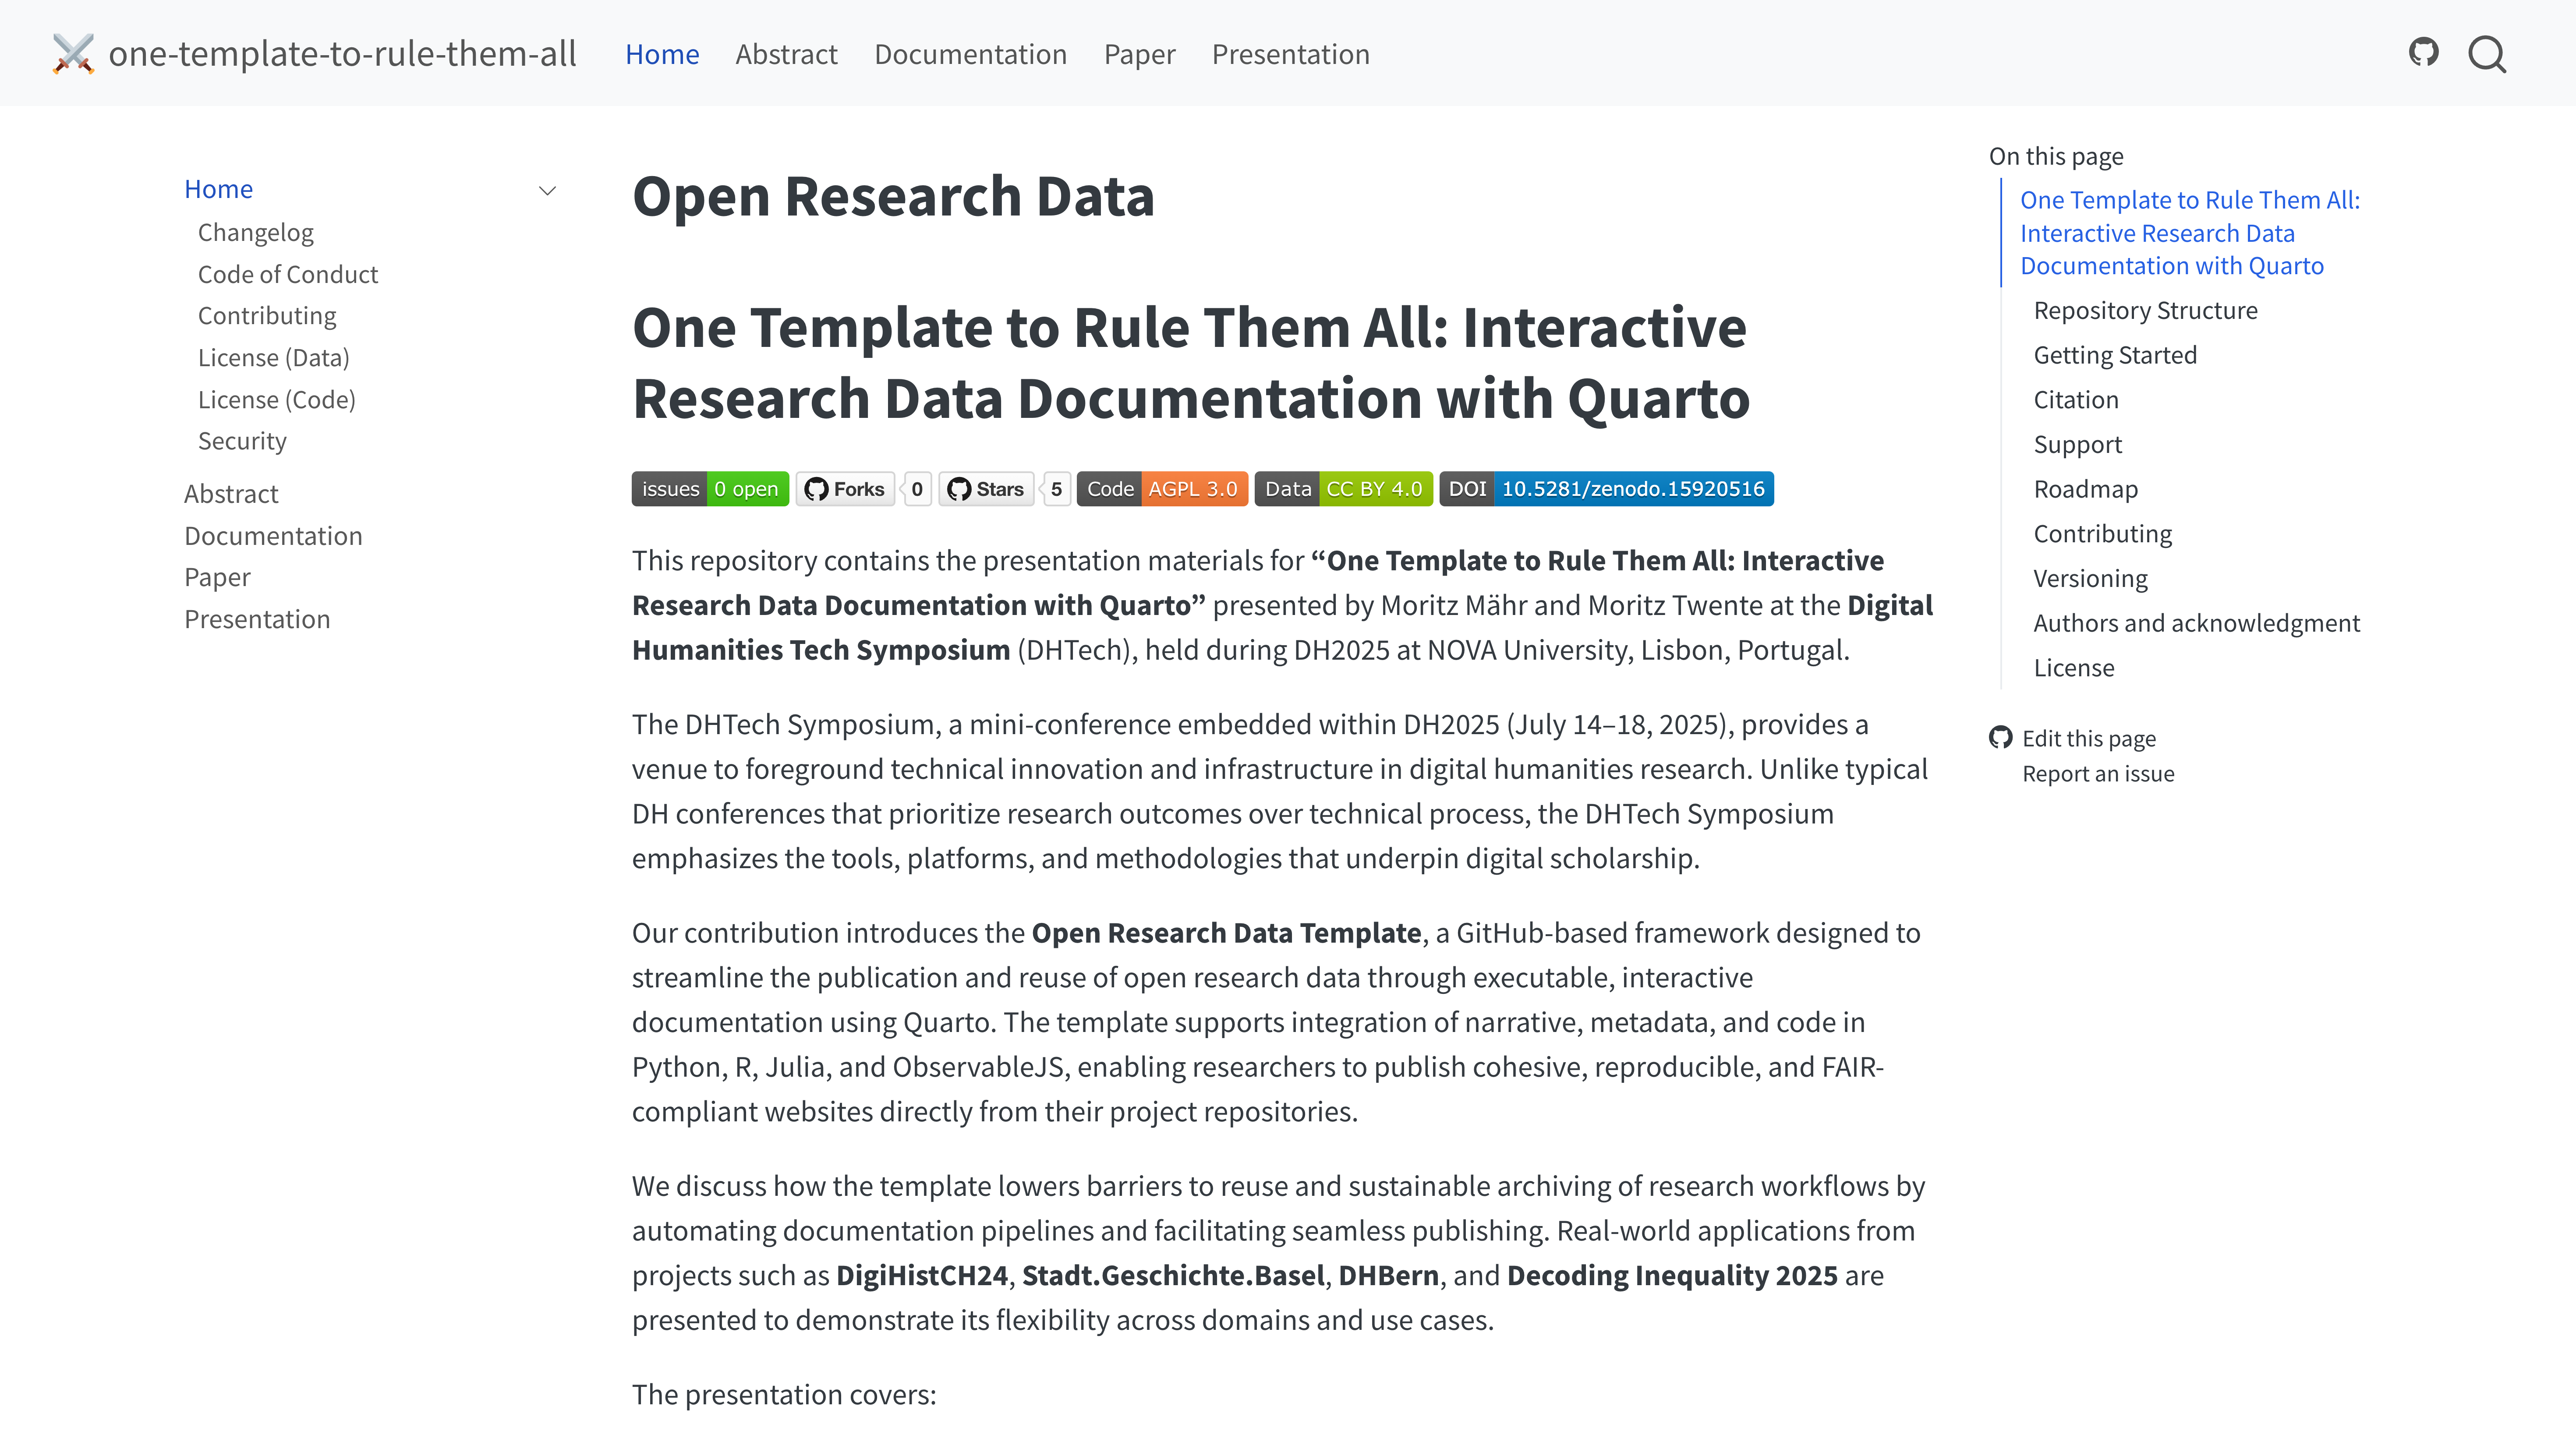
\includegraphics[width=0.9\linewidth]{images/one_template_to_rule_them_all.png}
  \caption{Landing page of the \emph{One Template to Rule Them All} project, presenting a framework for interactive research data documentation with Quarto.}
  \label{fig-one-template}
\end{figure}

Across all these use cases, a pattern emerges: the Open Research Data Template helped make sound RDM and open science practices easier to implement by packaging them into a reusable toolkit. Whether it was a large public history project, a standalone dataset publication, a collaborative handbook, or a course website, the template provided a backbone to ensure that the outputs were accessible, reproducible, and sustainable. Each deployment also fed back into the project -- for example, the need to support multiple output formats became clear with the handbook and presentation, which led us to refine how the template's configuration handled HTML/PDF/Word generation and slides. In this way, continuous use has been a form of continuous development.

\section{Conclusion}\label{conclusion}

Our experience with the Stadt.Geschichte.Basel project and the subsequent development of the Open Research Data Template highlights the value of making robust, interactive documentation a standard component of research data management. By lowering technical barriers, we made it as easy as possible for researchers (and ourselves) to follow best practices in open data: the template abstracts the complexities of web publishing, reproducibility, and archiving into a user-friendly workflow. This means historians and humanities scholars -- who might not be seasoned programmers -- can still produce state-of-the-art research outputs that are transparent and reusable. Crucially, the use of static-site technology (Quarto + GitHub Pages) contributes to sustainability (noting that while we do lock into the Microsoft universe by using GitHub as a platform, we also help cement its place as a de facto marketplace for open source code). Static sites are lightweight, secure (no moving parts on the server), and likely to remain accessible years into the future with minimal maintenance. They can be archived in repositories like Zenodo, preserving not just the data but the complete context needed to understand and reuse that data.

In sum, good interactive documentation is not an added bonus but a fundamental part of making research data truly open and useful. Our template empowers projects to create ``living'' documentation that keeps data, code, and narrative in sync, which we believe is a key ingredient for impactful and reproducible Digital Humanities research. The positive reception and diverse adoption of the template across use cases indicate that this approach resonates with the needs of the community. We argue that initiatives like ours help shift the culture toward treating research outputs as dynamic resources to be explored and built upon, rather than static end products. By combining modern open-source tools and best practices, and by focusing on ease of use, we hope to see more researchers embrace these methods. Ultimately, making open research data practices easy and even automatic frees scholars to focus on the content of their research, while ensuring that their work can endure, be understood, and inspire future work in the years to come.

\section*{Acknowledgements}

This unnumbered section should be blank when submitting your paper. After review, you may include lists of people and organizations who supported the work.

% Print the biblography at the end. Keep this line after the main text of your paper, and before an appendix. 
\printbibliography

% You can include an appendix using the following command
% \appendix

% \section{First Appendix Section} \label{appdx:first}

% Appendix sections should be ordered by letters rather than numbers, and their contents do not count towards the paper's length limit. Appendix sections may also contain additional tables and figures.  

\end{document}